% !TeX root = ../main.tex

\section{Data set}
The Epinions data set \citep{Massa} is a very good case to demonstrate the Recursive
K-Nearest Neighbors algorithm because of its sparsity. As demonstrated in \autoref{chap:3},
this algorithm manages to overcome the limitations of the conventional KNN algorithm, which
cannot make predictions for ratings with no direct associations to other users or items.
This dataset consists of 40163 users and 139738 items and 664824 ratings.
As we mentioned previously, the sparsity percentage is 0,99988154.
The structure of the dataset is shown in the table below:
\begin{table}[H]
\centering
\caption{Epinions Dataset Sample}
\label{table:Epinions_sample}
\begin{tabular}{ |c|c|c| }
\hline
\textbf{user} & \textbf{item} & \textbf{Rating} \\
\hline
36153 & 62461 & 5 \\
\hline
427 & 38005 & 5  \\
\hline
751 & 53361 & 4 \\
\hline
11001 & 118950 & 4 \\
\hline
1169 & 66176 & 5 \\
\hline
9808 & 84459 & 2 \\
\hline
85 & 7446 & 4 \\
\hline
14717 & 3397 & 2 \\
\hline
\end{tabular}
\end{table}
The user and item columns contain the ids of users and items respectively, and the rating
column contains the rating of a user to an item. To test the accuracy of
KNN and Recursive-KNN algorithms this ratings matrix was split in a
train set and a test set. The train set is used so the algorithms can learn the
patterns of the data. Either how users rate or how items are being rated.
The similarity metrics discussed in \autoref{chap:2} will be computed based on
the train set and the rating predictions will be calculated based on this set's
ratings. The rating predictions will be both user-based and item based.
The test set is used to evaluate the rating predictions produced by the trained algorithms
to this set using an aggregating error function between the predictions
and the truth values. The train set consists of 520203
ratings(78\%) and the test set consists of 144621 ratings(22\%). The train
set is stratified by users, which means that it contains a proportion of each
user's ratings. Below there are some descriptive information about the Epinions dataset and the splitting method.
\begin{table}[H]
\centering
\caption{Epinions Descriptive}
\label{table:epinions_descriptive}
\begin{tabular}{ |c|c|c|c| }
\hline
&\textbf{Ratings Matrix} & \textbf{Train} & \textbf{Test}\\
\hline
count & 664824 & 520203 & 144621\\
\hline
mean & 3.9917 & 3.99 & 3.9975\\
\hline
std & 1.2068 & 1.2072 & 1.2053\\
\hline
min & 1 & 1 & 1\\
\hline
25\% & 3 & 3 & 3\\
\hline
50\% & 4 & 4 & 4\\
\hline
75\% & 5 & 5 & 5\\
\hline
max & 5 & 5 & 5\\
\hline
\end{tabular}
\end{table}

In the subsections below we present some basic descriptive information about each of the similarity
methods and in \autoref{sec:4.3} we will present the best result from the
rating predictions.

\subsection{Cosine Similarity}

\begin{figure}[H]
\centering
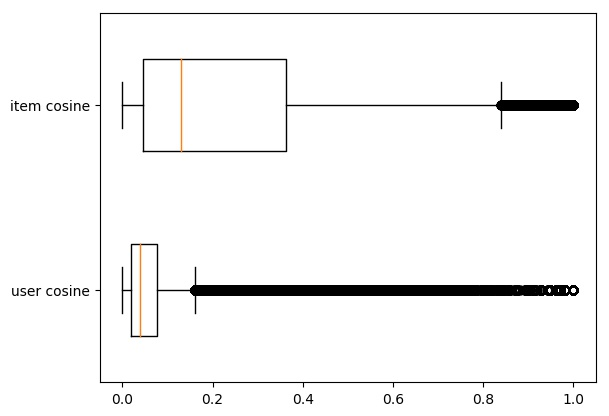
\includegraphics[width=0.7\textwidth]{chapter_4/boxplots/cosine/cosine_boxplot.jpg}
\caption{Cosine Similarity Boxplot (Whiskers= -+1.5IQR)}
\label{figure:cosine_similarity_boxplot}
\end{figure}

Both item and user similarity values have a minimum value near zero.The items' right whisker value is
around 0.8 and the users' around 0.18. Both items and users similarity outliers seem to reach the value of 1.
Also the number of outliers in item cosine appears significantly lower than that of the users.
At least 75\% of users similarities are lower than 0.1. In contrast, at least 50\% of
item similarities are larger than 0.1 and at least 25\% are larger than 0.35.

\begin{table}[H]
\centering
\caption{Cosine Similarity Descriptive}
\label{table:cosine_similarity_descriptive}
\begin{tabular}{|c|c|c|}
\hline
		  & \textbf{users} & \textbf{items} \\ \hline
count     & 14614164       & 18672616       \\ \hline
mean      & 0.063717709    & 0.2590515005   \\ \hline
std       & 0.0852396246   & 0.2948759498   \\ \hline
min       & 0.0001118907   & 0.0001876405   \\ \hline
25\%      & 0.0184512236   & 0.0467473495   \\ \hline
50\%      & 0.0389925088   & 0.1290322581   \\ \hline
75\%      & 0.0758098044   & 0.3638034376   \\ \hline
max       & 1              & 1              \\ \hline
max count & 26742          & 1519527        \\ \hline
min count & 1              & 1              \\ \hline
\end{tabular}
\end{table}

\begin{table}[H]
\centering
\caption{Cosine Similarity Count Descriptive}
\label{table:cosine_similarity_count_descriptive}
\begin{tabular}{|c|c|c|}
\hline
          & \textbf{users}  & \textbf{items} \\ \hline
count     & 39156           & 121140         \\ \hline
mean      & 746.4584737971  & 308.281591547  \\ \hline
std       & 1174.5013754664 & 666.5799806645 \\ \hline
min       & 1               & 1              \\ \hline
25\%      & 40              & 37             \\ \hline
50\%      & 246             & 120            \\ \hline
75\%      & 944             & 338            \\ \hline
max       & 13843           & 31057          \\ \hline
max count & 1               & 1              \\ \hline
min count & 793             & 545            \\ \hline
\end{tabular}
\end{table}

\subsection{Modified Cosine Similarity}

\begin{figure}[H]
\centering
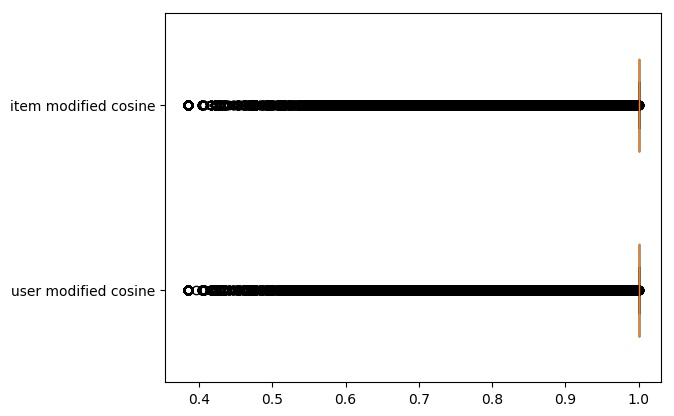
\includegraphics[width=0.9\textwidth]{chapter_4/boxplots/modified_cosine/modified_cosine_boxplot.jpg}
\caption{Modified Cosine Similarity Boxplot (Whiskers= -+1.5IQR)}
\label{figure:modified_cosine_similarity_boxplot}
\end{figure}

Modified cosine similarity seems to have the same effect in the values for both items
and users. Both these boxplots have the majority of their values at 1. Their minimum values
are a little less than 0.4. Any value other than 1 can be interpreted as an outlier.

\begin{table}[H]
\centering
\caption{Modified Cosine Similarity Descriptive}
\label{table:modified_cosine_similarity_descriptive}
\begin{tabular}{|c|c|c|}
\hline
          & \textbf{users} & \textbf{items} \\ \hline
count     & 14614164       & 18672616       \\ \hline
mean      & 0.9923727737   & 0.9970178776   \\ \hline
std       & 0.0345699768   & 0.0205710501   \\ \hline
min       & 0.3846153846   & 0.3846153846   \\ \hline
25\%      & 1              & 1              \\ \hline
50\%      & 1              & 1              \\ \hline
75\%      & 1              & 1              \\ \hline
max       & 1              & 1              \\ \hline
max count & 12887451       & 17728374       \\ \hline
min count & 1170           & 263            \\ \hline
\end{tabular}
\end{table}

\begin{table}[H]
\centering
\caption{Modified Cosine Similarity Count Descriptive}
\label{table:modified_cosine_similarity_count_descriptive}
\begin{tabular}{|c|c|c|}
\hline
          & \textbf{users}  & \textbf{items} \\ \hline
count     & 39156           & 121140         \\ \hline
mean      & 746.4584737971  & 308.281591547  \\ \hline
std       & 1174.5013754664 & 666.5799806645 \\ \hline
min       & 1               & 1              \\ \hline
25\%      & 40              & 37             \\ \hline
50\%      & 246             & 120            \\ \hline
75\%      & 944             & 338            \\ \hline
max       & 13843           & 31057          \\ \hline
max count & 1               & 1              \\ \hline
min count & 793             & 545            \\ \hline
\end{tabular}
\end{table}

\subsection{Adjusted Cosine Similarity}

\begin{figure}[H]
\centering
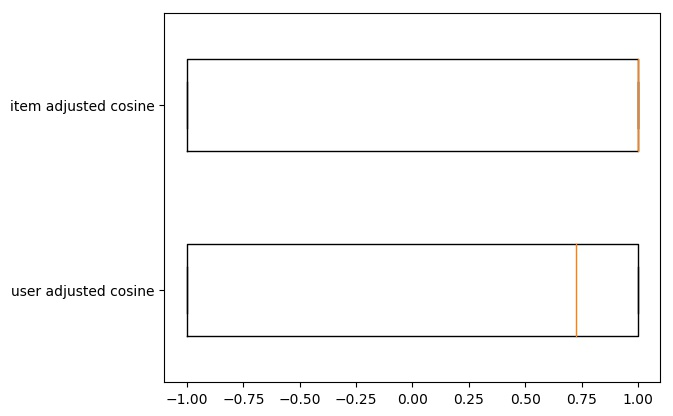
\includegraphics[width=0.8\textwidth]{chapter_4/boxplots/adjusted_cosine/adjusted_cosine_boxplot.jpg}
\caption{Adjusted Cosine Similarity Boxplot (Whiskers= -+1.5IQR)}
\label{figure:adjusted_cosine_similarity_boxplot}
\end{figure}

Adjusted cosine similarity seems to have distributed the values both for users and items very well.
There are no outliers for either of these boxplots. Although, items have at least 50\% of their
values at 1, users have at least 50\% of their values over 0.7. They both have their minimum
value at -1.

\begin{table}[H]
\centering
\caption{Adjusted Cosine Similarity Descriptive}
\label{table:adjusted_cosine_similarity_descriptive}
\begin{tabular}{|c|c|c|}
\hline
          & \textbf{users} & \textbf{items} \\ \hline
count     & 14547343       & 18578462       \\ \hline
mean      & 0.073856558    & 0.09784622     \\ \hline
std       & 0.9611564664   & 0.9793750112   \\ \hline
min       & -1             & -1             \\ \hline
25\%      & -1             & -1             \\ \hline
50\%      & 0.7255719661   & 1              \\ \hline
75\%      & 1              & 1              \\ \hline
max       & 1              & 1              \\ \hline
max count & 6998746        & 9729527        \\ \hline
min count & 5753489        & 7845237        \\ \hline
\end{tabular}
\end{table}

\begin{table}[H]
\centering
\caption{Adjusted Cosine Similarity Count Descriptive}
\label{adjusted_cosine_similarity_count_descriptive}
\begin{tabular}{|c|c|c|}
\hline
          & \textbf{users}  & \textbf{items} \\ \hline
count     & 38302           & 119634         \\ \hline
mean      & 759.6127095191  & 310.5883277329 \\ \hline
std       & 1179.0168839062 & 666.8475091836 \\ \hline
min       & 1               & 1              \\ \hline
25\%      & 45              & 39             \\ \hline
50\%      & 260             & 123            \\ \hline
75\%      & 968             & 340            \\ \hline
max       & 13798           & 30920          \\ \hline
max count & 1               & 1              \\ \hline
min count & 569             & 398            \\ \hline
\end{tabular}
\end{table}

\subsection{Modified Adjusted Cosine Similarity}

\begin{figure}[H]
\centering
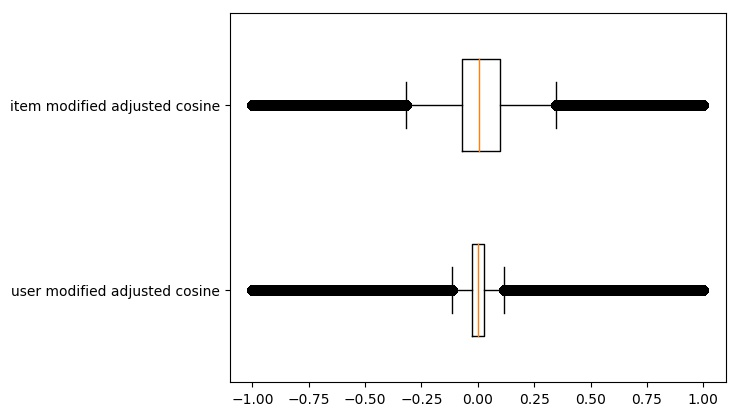
\includegraphics[width=0.8\textwidth]{chapter_4/boxplots/modified_adjusted_cosine/modified_adjusted_cosine_boxplot.jpg}
\caption{Modified Adjusted Cosine Similarity Boxplot (Whiskers= -+1.5IQR)}
\label{figure:modified_adjusted_cosine_similarity_boxplot}
\end{figure}

The modification used in adjusted cosine similarity seems to have enclosed the values near zero.
Their median is aligned very close to zero. The whiskers for items are around -0.4 and 0.4
for left and right respectively. For users, the whiskers are around -0.12 and 0.12 for left and right
respectively. Items similarities behave like a wider version of users similarities, probably
because items are more than twice the size of users which allows them to form a wider range of
different similarities.

\begin{table}[H]
\centering
\caption{Modified Adjusted Cosine Similarity Descriptive}
\label{table:modified_adjusted_cosine_similarity_descriptive}
\begin{tabular}{|c|c|c|}
\hline
          & \textbf{users} & \textbf{items} \\ \hline
count     & 14547343       & 18578462       \\ \hline
mean      & 0.0004873924   & 0.0165982167   \\ \hline
std       & 0.1313835099   & 0.398039276    \\ \hline
min       & -1             & -1             \\ \hline
25\%      & -0.0280684821  & -0.0701974943  \\ \hline
50\%      & 0.0012377237   & 0.0033406502   \\ \hline
75\%      & 0.029188451    & 0.096874534    \\ \hline
max       & 1              & 1              \\ \hline
max count & 17005          & 863028         \\ \hline
min count & 11891          & 679602         \\ \hline
\end{tabular}
\end{table}

\begin{table}[H]
\centering
\caption{Modified Adjusted Cosine Similarity Count Descriptive}
\label{table:modified_adjusted_cosine_similarity_count_descriptive}
\begin{tabular}{|c|c|c|}
\hline
          & \textbf{users}  & \textbf{items} \\ \hline
count     & 38302           & 119634         \\ \hline
mean      & 759.6127095191  & 310.5883277329 \\ \hline
std       & 1179.0168839062 & 666.8475091836 \\ \hline
min       & 1               & 1              \\ \hline
25\%      & 45              & 39             \\ \hline
50\%      & 260             & 123            \\ \hline
75\%      & 968             & 340            \\ \hline
max       & 13798           & 30920          \\ \hline
max count & 1               & 1              \\ \hline
min count & 569             & 398            \\ \hline
\end{tabular}
\end{table}

\subsection{Pearson Correlation Coefficient}

\begin{figure}[H]
\centering
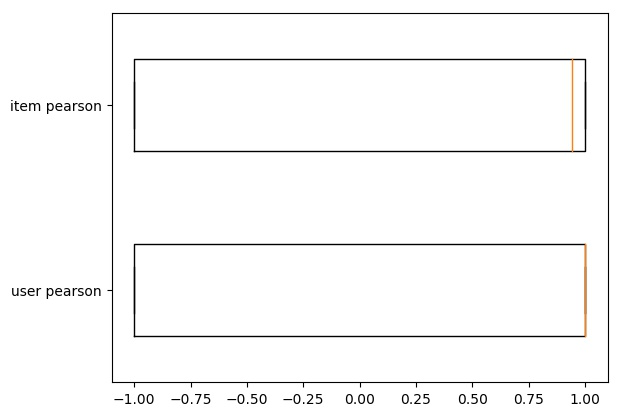
\includegraphics[width=0.8\textwidth]{chapter_4/boxplots/pearson/pearson_boxplot.jpg}
\caption{Pearson Correlation Coefficient Boxplot (Whiskers= -+1.5IQR)}
\label{figure:pearson_corr_coef_boxplot}
\end{figure}

The similarities formed using the Pearson correlation coefficient seem well distributed across
the range -1 to 1. No outliers exist in both users and items. In the users' boxplot at least 50\% of the
values appear to be near 1. In the items' boxplot at least 50\% of the values are over 0.8. The
minimum value for both of the similarities is at -1.

\begin{table}[H]
\centering
\caption{Pearson Correlation Coefficient Descriptive}
\label{table:pearson_corr_coef_descriptive}
\begin{tabular}{|c|c|c|}
\hline
          & \textbf{users} & \textbf{items} \\ \hline
count     & 12801832       & 9114131        \\ \hline
mean      & 0.2437009881   & 0.0973284577   \\ \hline
std       & 0.9285318435   & 0.9625193963   \\ \hline
min       & -1             & -1             \\ \hline
25\%      & -1             & -1             \\ \hline
50\%      & 1              & 0.940706152    \\ \hline
75\%      & 1              & 1              \\ \hline
max       & 1              & 1              \\ \hline
max count & 6825146        & 4489219        \\ \hline
min count & 4163467        & 3678485        \\ \hline
\end{tabular}
\end{table}

\begin{table}[H]
\centering
\caption{Pearson Correlation Coefficient Count Descriptive}
\label{table:pearson_corr_coef_boxplot}
\begin{tabular}{|c|c|c|}
\hline
          & \textbf{users}  & \textbf{items} \\ \hline
count     & 26166           & 40409          \\ \hline
mean      & 978.5089046855  & 451.0941126977 \\ \hline
std       & 1227.2905909627 & 753.2523780236 \\ \hline
min       & 1               & 1              \\ \hline
25\%      & 148             & 90             \\ \hline
50\%      & 507             & 222            \\ \hline
75\%      & 1353            & 500            \\ \hline
max       & 12486           & 17515          \\ \hline
max count & 1               & 1              \\ \hline
min count & 89              & 16             \\ \hline
\end{tabular}
\end{table}

\subsection{Pearson Modification 1}

\begin{figure}[H]
\centering
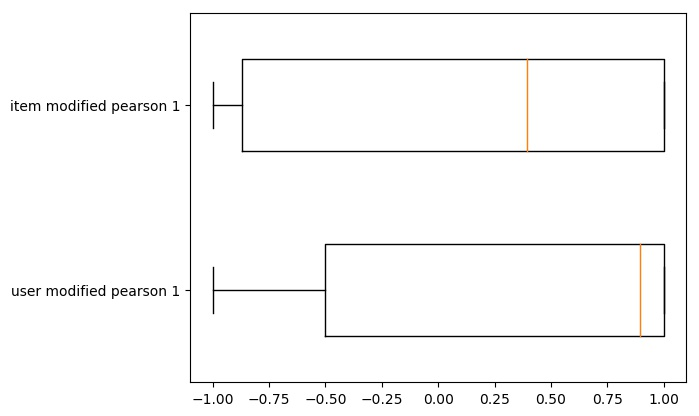
\includegraphics[width=0.8\textwidth]{chapter_4/boxplots/modified_pearson_1/modified_pearson_1_boxplot.jpg}
\caption{Modified Pearson 1 Boxplot (Whiskers= -+1.5IQR)}
\label{figure:modified_pearson_1_boxplot}
\end{figure}

The minimum value for both users and items similarities is at -1. Users have at least 50\% of their
values over 0.8 and at least 25\% at 1. Items' median is around 0.4. Items also seem to have
a 25\% of their value at 1. Both have their minimum at -1. At least 25\% of the similarities
for both users and items are negative.

\begin{table}[H]
\centering
\caption{Modified Pearson 1 Descriptive}
\label{table:modified_pearson_1_descriptive}
\begin{tabular}{|c|c|c|}
\hline
          & \textbf{users} & \textbf{items} \\ \hline
count     & 1161526        & 560066         \\ \hline
mean      & 0.3619158933   & 0.1343440987   \\ \hline
std       & 0.8153387654   & 0.8305601334   \\ \hline
min       & -1             & -1             \\ \hline
25\%      & -0.5           & -0.8703882798  \\ \hline
50\%      & 0.8947368421   & 0.3942210015   \\ \hline
75\%      & 1              & 1              \\ \hline
max       & 1              & 1              \\ \hline
max count & 529709         & 184408         \\ \hline
min count & 227880         & 133046         \\ \hline
\end{tabular}
\end{table}

\begin{table}[H]
\centering
\caption{Modified Pearson 1 Count Descriptive}
\label{modified_pearson_1_count_descriptive}
\begin{tabular}{|c|c|c|}
\hline
          & \textbf{users} & \textbf{items} \\ \hline
count     & 19566          & 25208          \\ \hline
mean      & 118.7290197281 & 44.4355760076  \\ \hline
std       & 266.6999446542 & 153.5700823656 \\ \hline
min       & 1              & 1              \\ \hline
25\%      & 5              & 2              \\ \hline
50\%      & 23             & 6              \\ \hline
75\%      & 105            & 24             \\ \hline
max       & 5003           & 5401           \\ \hline
max count & 1              & 1              \\ \hline
min count & 2066           & 5234           \\ \hline
\end{tabular}
\end{table}


\subsection{Pearson Modification 2}
\begin{figure}[H]
\centering
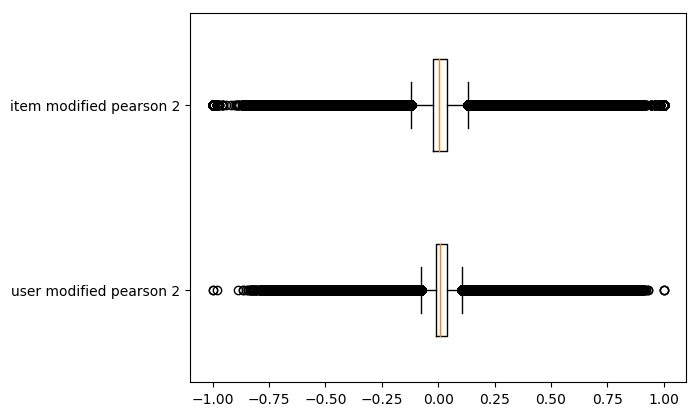
\includegraphics[width=0.8\textwidth]{chapter_4/boxplots/modified_pearson_2/modified_pearson_2_boxplot.jpg}
\caption{Modified Pearson 2 Boxplot (Whiskers= -+1.5IQR)}
\label{figure:modified_pearson_2_boxplot}
\end{figure}

At a first glance, these boxplots look very similar to \autoref{figure:modified_adjusted_cosine_similarity_boxplot}.
This is probably because the modification in both cases was to include the entire vectors in the
denominator (see \autoref{eq:modified_adjusted_cosine} and \autoref{eq:pearson_2}). Both boxplots have
their median near zero. They both have many outliers that spread both left and right of the boxes with
minimum value at -1 and maximum at 1. The whiskers are around -0.2 to -0.15 from the left
side and 0.15 to 0.2 from the right side.

\begin{table}[H]
\centering
\caption{Modified Pearson 2 Descriptive}
\label{table:modified_pearson_2_descriptive}
\begin{tabular}{|c|c|c|}
\hline
          & \textbf{users} & \textbf{items} \\ \hline
count     & 12801832       & 9114131        \\ \hline
mean      & 0.0218434042   & 0.0101521404   \\ \hline
std       & 0.089326644    & 0.1385987076   \\ \hline
min       & -1             & -1             \\ \hline
25\%      & -0.0093795851  & -0.0251329949  \\ \hline
50\%      & 0.0076098072   & 0.0037092894   \\ \hline
75\%      & 0.0367446145   & 0.0372677996   \\ \hline
max       & 1              & 1              \\ \hline
max count & 3              & 710            \\ \hline
min count & 2              & 412            \\ \hline
\end{tabular}
\end{table}

\begin{table}[H]
\centering
\caption{Modified Pearson 2 Count Descriptive}
\label{table:modified_pearson_2_count_descriptive}
\begin{tabular}{|c|c|c|}
\hline
          & \textbf{users}  & \textbf{items} \\ \hline
count     & 26166           & 40409          \\ \hline
mean      & 978.5089046855  & 451.0941126977 \\ \hline
std       & 1227.2905909627 & 753.2523780236 \\ \hline
min       & 1               & 1              \\ \hline
25\%      & 148             & 90             \\ \hline
50\%      & 507             & 222            \\ \hline
75\%      & 1353            & 500            \\ \hline
max       & 12486           & 17515          \\ \hline
max count & 1               & 1              \\ \hline
min count & 89              & 16             \\ \hline
\end{tabular}
\end{table}

\subsection{MSD}
\begin{figure}[H]
\centering
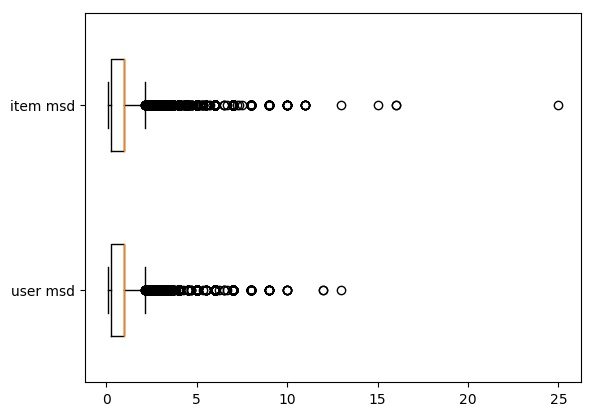
\includegraphics[width=0.8\textwidth]{chapter_4/boxplots/msd/msd_boxplot.jpg}
\caption{MSD Boxplot (Whiskers= -+1.5IQR)}
\label{figure:msd_boxplot}
\end{figure}

The minimum similarity value for both users and items is very close to zero. Their median
is around 1 and 75\% of the similarities are below 2. They both have a lot of outliers that
reach a score around 15. Item similarity has some more extreme outliers that are very close to 25.

\begin{table}[H]
\centering
\caption{MSD Descriptive}
\label{table:msd_descriptive}
\begin{tabular}{|c|c|c|}
\hline
          & \textbf{users} & \textbf{items} \\ \hline
count     & 9805108        & 12434536       \\ \hline
mean      & 0.6661864961   & 0.6544694584   \\ \hline
std       & 0.5256923021   & 0.4628208708   \\ \hline
min       & 0.0625         & 0.0625         \\ \hline
25\%      & 0.25           & 0.25           \\ \hline
50\%      & 1              & 1              \\ \hline
75\%      & 1              & 1              \\ \hline
max       & 13             & 25             \\ \hline
max count & 1              & 1              \\ \hline
min count & 598720         & 800571         \\ \hline
\end{tabular}
\end{table}

\begin{table}[H]
\centering
\caption{MSD Count Descriptive}
\label{msd_count_descriptive}
\begin{tabular}{|c|c|c|}
\hline
          & \textbf{users} & \textbf{items} \\ \hline
count     & 38442          & 120382         \\ \hline
mean      & 510.1247593778 & 206.5846388995 \\ \hline
std       & 850.5223750077 & 484.7004513454 \\ \hline
min       & 1              & 1              \\ \hline
25\%      & 25             & 22             \\ \hline
50\%      & 156            & 72             \\ \hline
75\%      & 613            & 213            \\ \hline
max       & 11014          & 23589          \\ \hline
max count & 1              & 1              \\ \hline
min count & 1182           & 1563           \\ \hline
\end{tabular}
\end{table}

\subsection{MAD}

\begin{figure}[H]
\centering
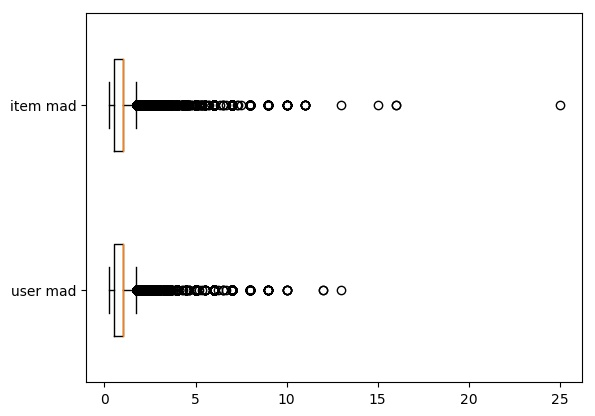
\includegraphics[width=0.8\textwidth]{chapter_4/boxplots/mad/mad_boxplot.jpg}
\caption{MAD Boxplot (Whiskers= -+1.5IQR)}
\label{figure:mad_boxplot}
\end{figure}

As expected, mean absolute difference boxplots are very similar to that of mean squared difference
\autoref{figure:msd_boxplot}. It is clear that the boxes have shrunk, due to the
fact that MAD uses the absolute values instead of the squared ones and this modification
lowers the standard deviation between the similarities.

\begin{table}[H]
\centering
\caption{MAD Descriptive}
\label{table:mad_descriptive}
\begin{tabular}{|c|c|c|}
\hline
          & \textbf{users} & \textbf{items} \\ \hline
count     & 9805108        & 12434536       \\ \hline
mean      & 0.7962500349   & 0.7668765592   \\ \hline
std       & 0.4338056858   & 0.3639417506   \\ \hline
min       & 0.25           & 0.25           \\ \hline
25\%      & 0.5            & 0.5            \\ \hline
50\%      & 1              & 1              \\ \hline
75\%      & 1              & 1              \\ \hline
max       & 13             & 25             \\ \hline
max count & 1              & 1              \\ \hline
min count & 598720         & 800571         \\ \hline
\end{tabular}
\end{table}

\begin{table}[H]
\centering
\caption{MAD Count Descriptive}
\label{table:mad_count_descriptive}
\begin{tabular}{|c|c|c|}
\hline
          & users          & items          \\ \hline
count     & 38442          & 120382         \\ \hline
mean      & 510.1247593778 & 206.5846388995 \\ \hline
std       & 850.5223750077 & 484.7004513454 \\ \hline
min       & 1              & 1              \\ \hline
25\%      & 25             & 22             \\ \hline
50\%      & 156            & 72             \\ \hline
75\%      & 613            & 213            \\ \hline
max       & 11014          & 23589          \\ \hline
max count & 1              & 1              \\ \hline
min count & 1182           & 1563			\\ \hline
\end{tabular}
\end{table}

\subsection{Jaccard Coefficient}
\begin{figure}[H]
\centering
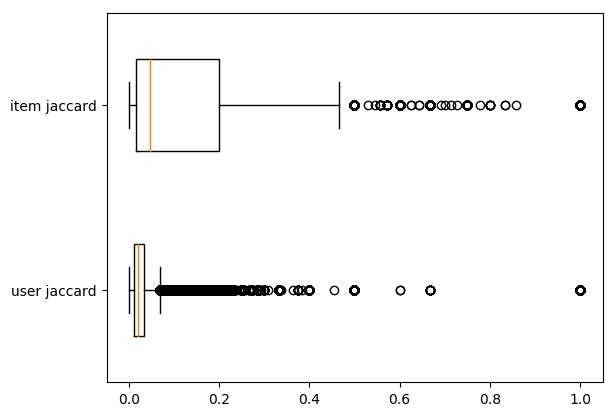
\includegraphics[width=0.8\textwidth]{chapter_4/boxplots/jaccard/jaccard_boxplot.jpg}
\caption{Jaccard Boxplot (Whiskers= -+1.5IQR)}
\label{figure:jaccard_boxplot}
\end{figure}

Both item and user similarity values have a minimum value near zero. The items' right whisker value is
around 0.45 and for the users around 0.04. Both items and users similarity outliers appear to reach the value
1. Also the number of outliers in item cosine seems significantly lower than users. At least 75\% of
users similarities are lower than 0.1. In contrast, at least 25\% of item similarities are larger than 0.2.
Users' boxplot is very narrow which indicates that 50\% of the values are very close to each other. It
covers a range of merely 0.02. On the other hand, the items' boxplot is relatively wider. It covers a range of about 0.19,
which confirms the wider spread of the values.

\begin{table}[H]
\centering
\caption{Jaccard Descriptive}
\label{table:jaccard_descriptive}
\begin{tabular}{|c|c|c|}
\hline
          & \textbf{users} & \textbf{items} \\ \hline
count     & 14614164       & 18672616       \\ \hline
mean      & 0.0307346429   & 0.1733928584   \\ \hline
std       & 0.0544456926   & 0.2779653358   \\ \hline
min       & 0.0006485084   & 0.0006060606   \\ \hline
25\%      & 0.0112359551   & 0.0153846154   \\ \hline
50\%      & 0.0196078431   & 0.0476190476   \\ \hline
75\%      & 0.0344827586   & 0.2            \\ \hline
max       & 1              & 1              \\ \hline
max count & 26746          & 1522328        \\ \hline
min count & 1              & 1              \\ \hline
\end{tabular}
\end{table}

\begin{table}[H]
\centering
\caption{Jaccard Count Descriptive}
\label{table:jaccard_count_descriptive}
\begin{tabular}{|c|c|c|}
\hline
          & \textbf{users}  & \textbf{items} \\ \hline
count     & 39156           & 121140         \\ \hline
mean      & 746.4584737971  & 308.281591547  \\ \hline
std       & 1174.5013754664 & 666.5799806645 \\ \hline
min       & 1               & 1              \\ \hline
25\%      & 40              & 37             \\ \hline
50\%      & 246             & 120            \\ \hline
75\%      & 944             & 338            \\ \hline
max       & 13843           & 31057          \\ \hline
max count & 1               & 1              \\ \hline
min count & 793             & 545            \\ \hline
\end{tabular}
\end{table}


\section{Evaluation Metrics}
The accuracy of the predictions is one of the most important goals in recommender
systems as it gives more chances that the prediction will be relevant to the
user. As discussed in \autoref{chap:1} other goals include the novelty of the
recommendations, serendipity and diversity. In this thesis the focus is
on the accuracy of the predictions. Four metrics will be discussed to evaluate the
Recursive Nearest Neighbors algorithm on the Epinions dataset.
\subsection{Root Mean Squared Error (RMSE)}
RMSE is one of the most popular accuracy estimators.
It sums the squared error between the true and estimated value divided by the
number of the predictions the model was able to extract. Finally it is square
rooted so that the error corresponds to units of ratings instead of square
units. \citep{Ricci}
$$RMSE = \sqrt{\frac{\sum_{(u,i) \in \mathcal{T}(r_{u,i} - \hat{r}_{u,i})^2}}{n}}$$
where,
\begin{itemize}
	\item[] $\mathcal{T}$ is the test set
	\item[] $r_{u,i}$ is the true rating of user $u$ to item $i$ in $\mathcal{T}$
	\item[] $\hat{r}_{u,i}$ is the rating prediction for user $u$ to item $i$
	\item[] $n$ is the number of predictions
\end{itemize}

\subsection{Mean Absolute Error (MAE)}
MAE is another popular metric for accuracy estimation. It sums the absolute
value between the difference between the true and estimated ratings
divided by the number of predictions. \citep{Ricci}
$$MAE = \frac{\sum_{(u,i) \in \mathcal{T}\left|r_{u,i} - \hat{r}_{u,i}\right|}}{n}$$
where,
\begin{itemize}
	\item[] $\mathcal{T}$ is the test set
	\item[] $r_{u,i}$ is the true rating of user $u$ to item $i$ in $\mathcal{T}$
	\item[] $\hat{r}_{u,i}$ is the rating prediction for user $u$ to item $i$
	\item[] $n$ is the number of predictions
\end{itemize}

\subsection{Mean Absolute User Error (MAUE)}
While RMSE and MAE estimate the global error to the system MAUE first
calculates the MAE score for each user then averages all user errors to find
how much the system diverges on average from each user \citep{Massa}.
$$MAUE = \frac{1}{n}\sum_{u \in \mathcal{T}}\frac{\sum_{i \in \mathcal{I}_u\mathopen|r_{u,i} - \hat{r}_{u,i}\mathclose|}}{n_u}$$
where,
\begin{itemize}
	\item[] $\mathcal{T}$ is the test set
	\item[] $r_{u,i}$ is the true rating of user $u$ to item $i$ in $\mathcal{T}$
	\item[] $\hat{r}_{u,i}$ is the rating prediction for user $u$ to item $i$
	\item[] $n_u$ is the number of predictions for user $u$
	\item[] $n$ is the number of users for whom predictions were made for
\end{itemize}
\subsection{Root Mean Squared User Error (RMSUE)}
Like in MAUE, the equation for RMSE can be used to produce a per user rmse estimate.
In this metric first the RMSE for every user is computed. Then the RMSEs of
the users are averaged to form the RMSUE score with is an estimate in the
error of the model per user of the dataset.
$$RMSUE = \frac{1}{n}\sum_{u \in \mathcal{T}}\sqrt{\frac{\sum_{i \in \mathcal{I}_u(y_{u,i} - \hat{y}_{u,i})^2}}{n_u}}$$
where,
\begin{itemize}
	\item[] $\mathcal{T}$ is the test set
	\item[] $r_{u,i}$ is the true rating of user $u$ to item $i$ in $\mathcal{T}$
	\item[] $\hat{r}_{u,i}$ is the rating prediction for user $u$ to item $i$
	\item[] $n_u$ is the number of predictions for user $u$
	\item[] $n$ is the number of users for whom predictions were made for
\end{itemize}

\section{Evaluation Results and Benchmarks}\label{sec:4.3}
For this experiment item-based and user-based similarities discussed in \autoref{chap:2} where used.
Any similarity metrics that could contain
negative similarities, had those negative similarities excluded from the
computations.
For the K-Nearest Neighbors, the following 22 different values
of $\mathcal{K}$ were used:
$$\mathcal{K} = [1, 3, 5, 10, 15, 20, 25, 30, 35, 40, 45, 50, 55, 60, 65, 70, 75, 80, 85, 90, 95, 100]$$
For the Recursive K-Nearest Neighbors, as defined in the
algorithmic steps of \autoref{chap:3}, 22 different values of $\mathcal{M}$
were also used:
$$\mathcal{M} = [1, 3, 5, 10, 15, 20, 25, 30, 35, 40, 45, 50, 55, 60, 65, 70, 75, 80, 85, 90, 95, 100]$$

Below, the best outcome based on each evaluation metric for user-based and
item-based CF will be presented. The combined errors for KNN and Recursive-KNN
for RMSE and MAE below are computed using these formulas:
\begin{itemize}
	\item[] \textbf{Total RMSE:}
	$$RMSE_{Total} = \sqrt{\frac{n_{KNN}*RMSE_{KNN}^2 + n_{R-KNN}*RMSE_{R-KNN}^2}{n_{KNN} + n_{R-KNN}}}$$
	where,
	\begin{itemize}
		\item[] $n_{KNN}$ is the number of predictions made using the KNN algorithm
		\item[] $RMSE_{KNN}$ is the RMSE score using the KNN algorithm
		\item[] $n_{R-KNN}$ is the number of predictions made using the Recursive KNN algorithm
		\item[] $RMSE_{R-KNN}$ is the RMSE score using the Recursive KNN algorithm
	\end{itemize}
	\item[] \textbf{Total MAE:}
	$$MAE_{Total} = \frac{n_{KNN}*MAE_{KNN} + n_{R-KNN}*MAE_{R-KNN}}{n_{KNN} + n_{R-KNN}}$$
	where,
	\begin{itemize}
		\item[] $n_{KNN}$ is the number of predictions made using the KNN algorithm
		\item[] $MAE_{KNN}$ is the MAE score using the KNN algorithm
		\item[] $n_{R-KNN}$ is the number of predictions made using the Recursive KNN algorithm
		\item[] $MAE_{R-KNN}$ is the MAE score using the Recursive KNN algorithm
	\end{itemize}
\end{itemize}

\autoref{chap:appendix_src} has a link to
the code written in Python(version 3.6) using the Anaconda distribution \citep{anaconda}
that calculated the similarities, rating predictions
and the errors. It also contains the train and test data, the \LaTeX{} structure
that this thesis was build on and the numerical results.
\autoref{chap:appendix_results} contains all the plots produced by the
numerical results. All plots in this thesis were produced using the Matplotlib library
\citep{Hunter:2007}.

\subsection{User-Based}
\begin{figure}[H]
\centering
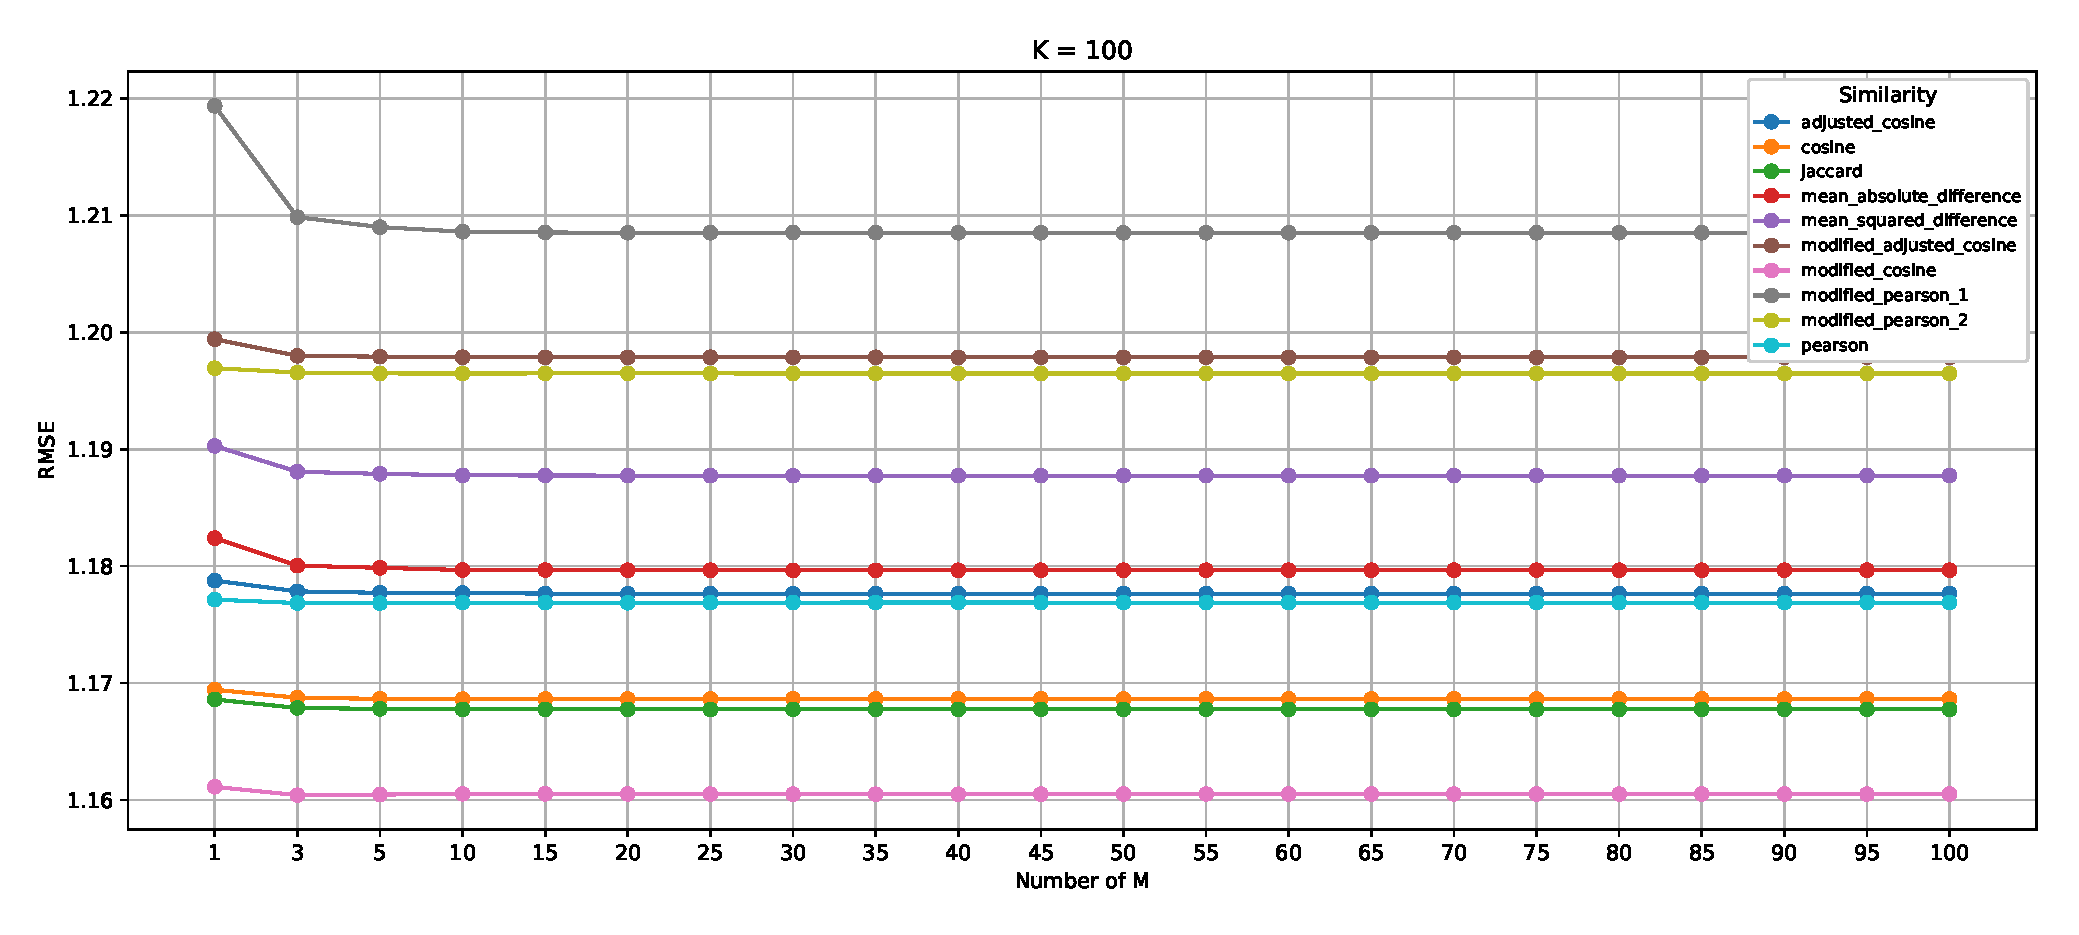
\includegraphics[width=1\textwidth]{chapter_4/evaluation/evaluation_user_rmse.eps}
\caption{User-based Total RMSE Best Score}
\label{figure:user_best_total_rmse}
\end{figure}
The best RMSE score for user-based CF was produced using $\mathcal{K}=100$ and $\mathcal{M}=3$.
The exact RMSE score is 1.1604146071 and it was calculated based on 124433 rating predictions(\autoref{table:prediction_counters_by_sim})
using the modified cosine similarity(\autoref{eq:modified_cosine})
for the 144621 ratings in the test set(\autoref{table:epinions_descriptive}).

\begin{figure}[H]
\centering
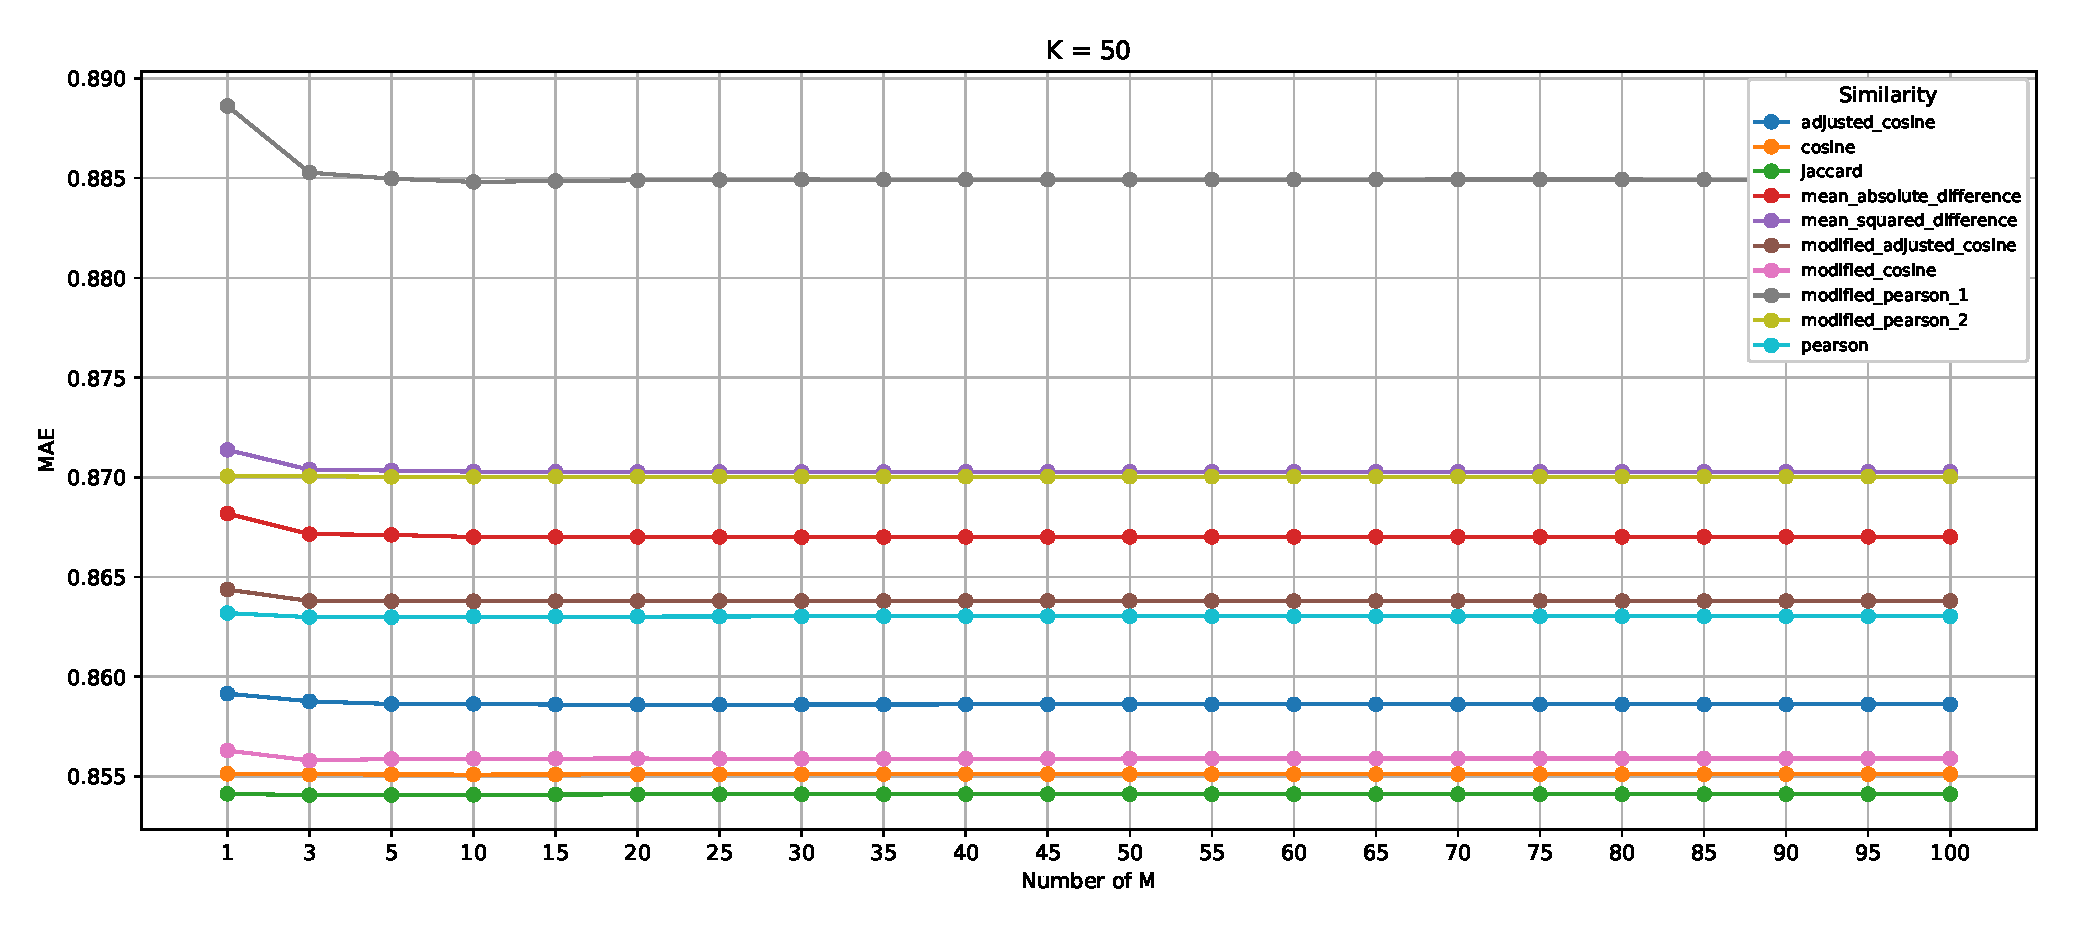
\includegraphics[width=1\textwidth]{chapter_4/evaluation/evaluation_user_mae.eps}
\caption{User-based Total MAE Best Score}
\label{figure:user_total_mae}
\end{figure}

The best MAE score for user-based CF was produced using $\mathcal{K}=50$ and $\mathcal{M}=3$.
The exact MAE score is 0.854066176 and it was calculated based on 124433 rating predictions(\autoref{table:prediction_counters_by_sim})
using the jaccard coefficient(\autoref{eq:jaccard})
for the 144621 ratings in the test set(\autoref{table:epinions_descriptive}).

\begin{figure}[H]
\centering
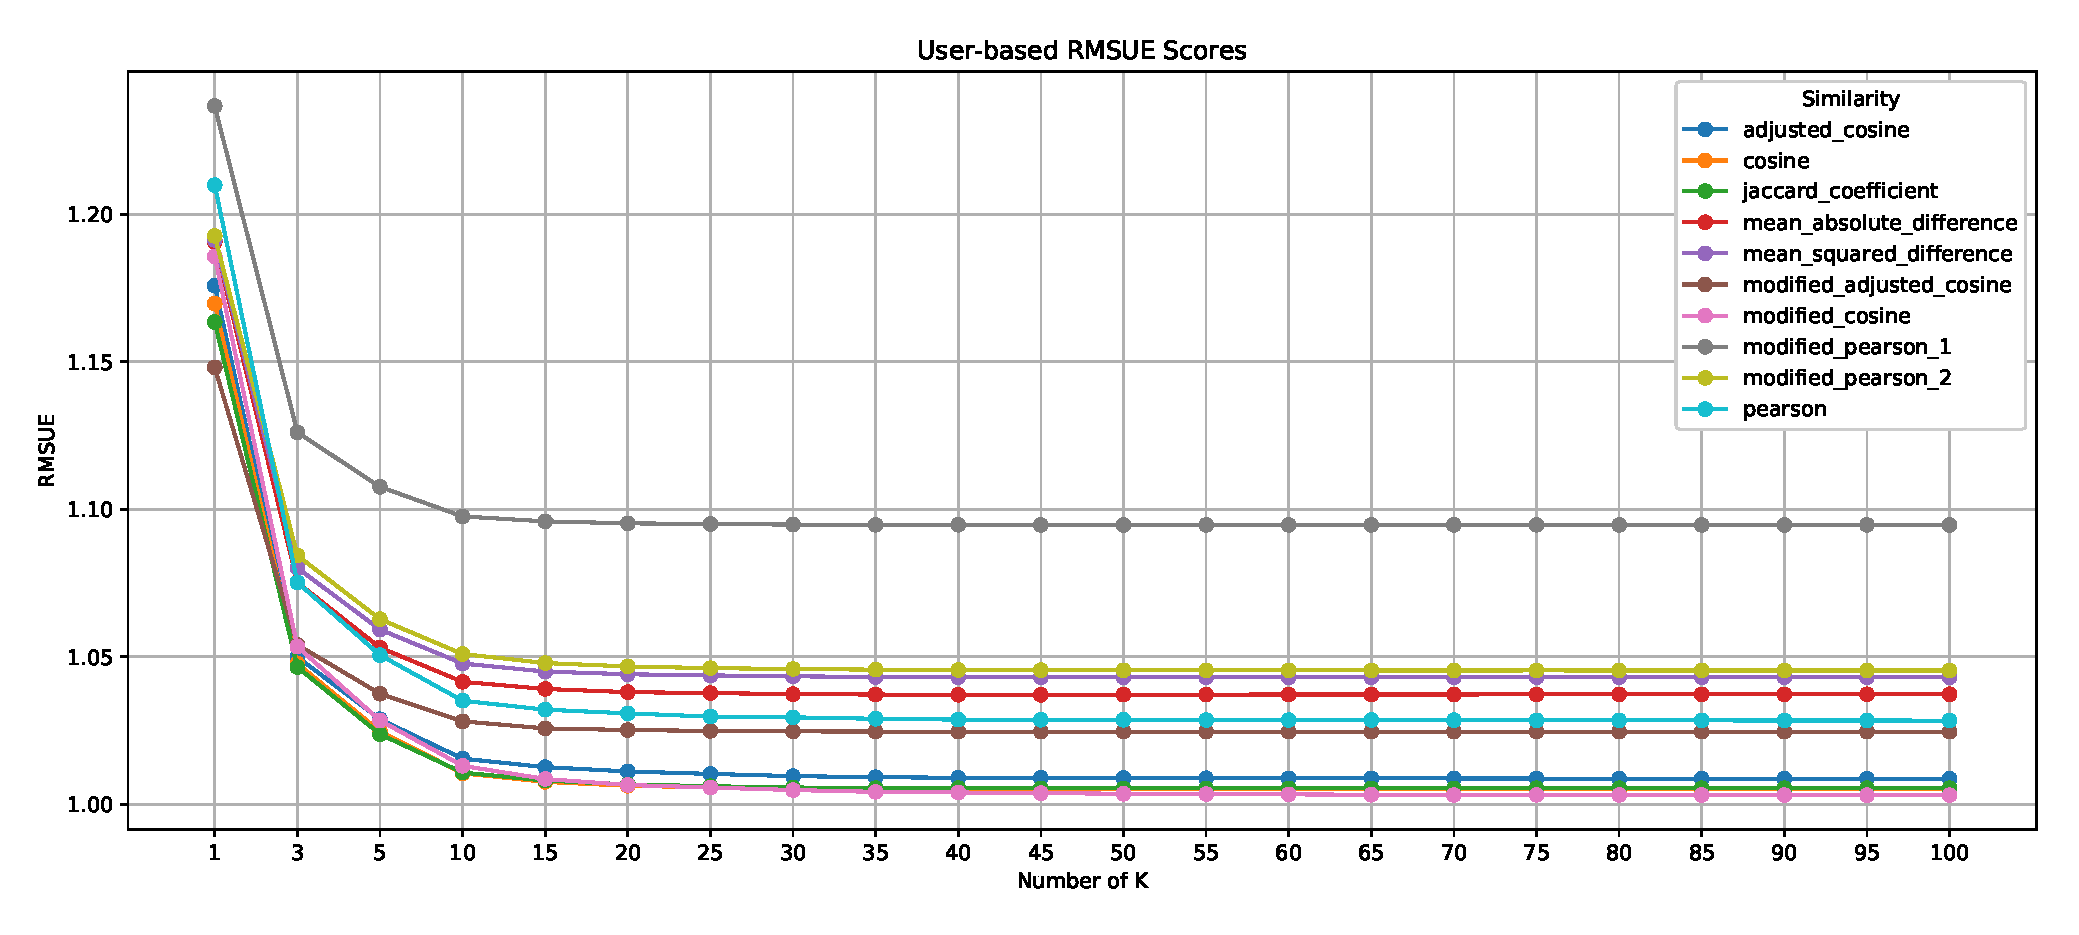
\includegraphics[width=1\textwidth]{chapter_4/knn/User_RMSUE_KNN.eps}
\caption{User-based KNN RMSUE Scores}
\label{figure:User_knn_rmsue}
\end{figure}

The best KNN RMSUE score for user-based CF was produced using $\mathcal{K}=100$.
The exact KNN RMSUE score is 1.0031145695 and it was calculated based on 100311 rating
predictions(\autoref{table:prediction_counters_by_sim})
using the modified cosine similarity(\autoref{eq:modified_cosine})
for the 144621 ratings in the test set(\autoref{table:epinions_descriptive}).

\begin{figure}[H]
\centering
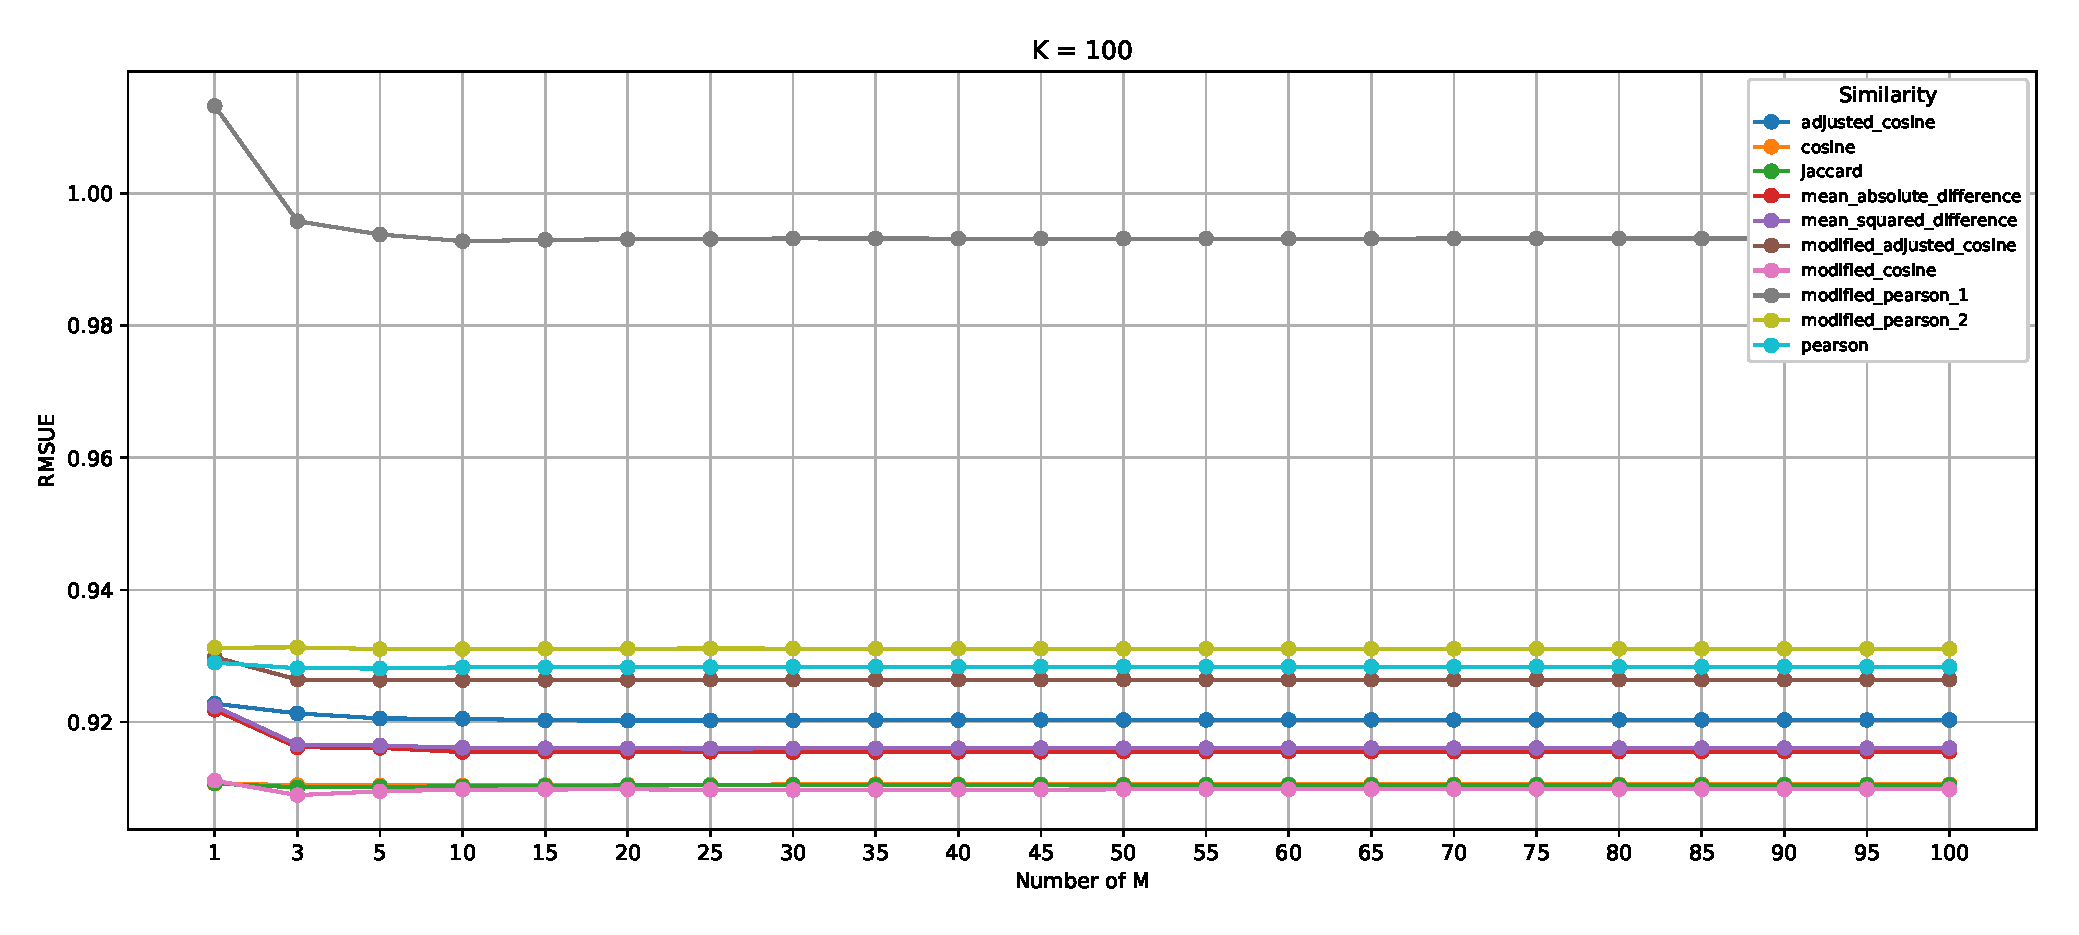
\includegraphics[width=1\textwidth]{chapter_4/evaluation/evaluation_user_rmsue.eps}
\caption{User-based Recursive-KNN RMSUE Best Score}
\label{figure:User_rknn_rmsue}
\end{figure}

The best Recursive-KNN RMSUE score for user-based CF was produced using $\mathcal{K}=100$ and $\mathcal{M}=3$.
The exact Recursive-KNN RMSUE score is 0.9089525549 and it was calculated based on 24122 rating
predictions(\autoref{table:prediction_counters_by_sim})
using the modified cosine similarity(\autoref{eq:modified_cosine})
out of the 25061 pairs for which KNN was unable to find neighbors(\autoref{table:users_log}).

\begin{figure}[H]
\centering
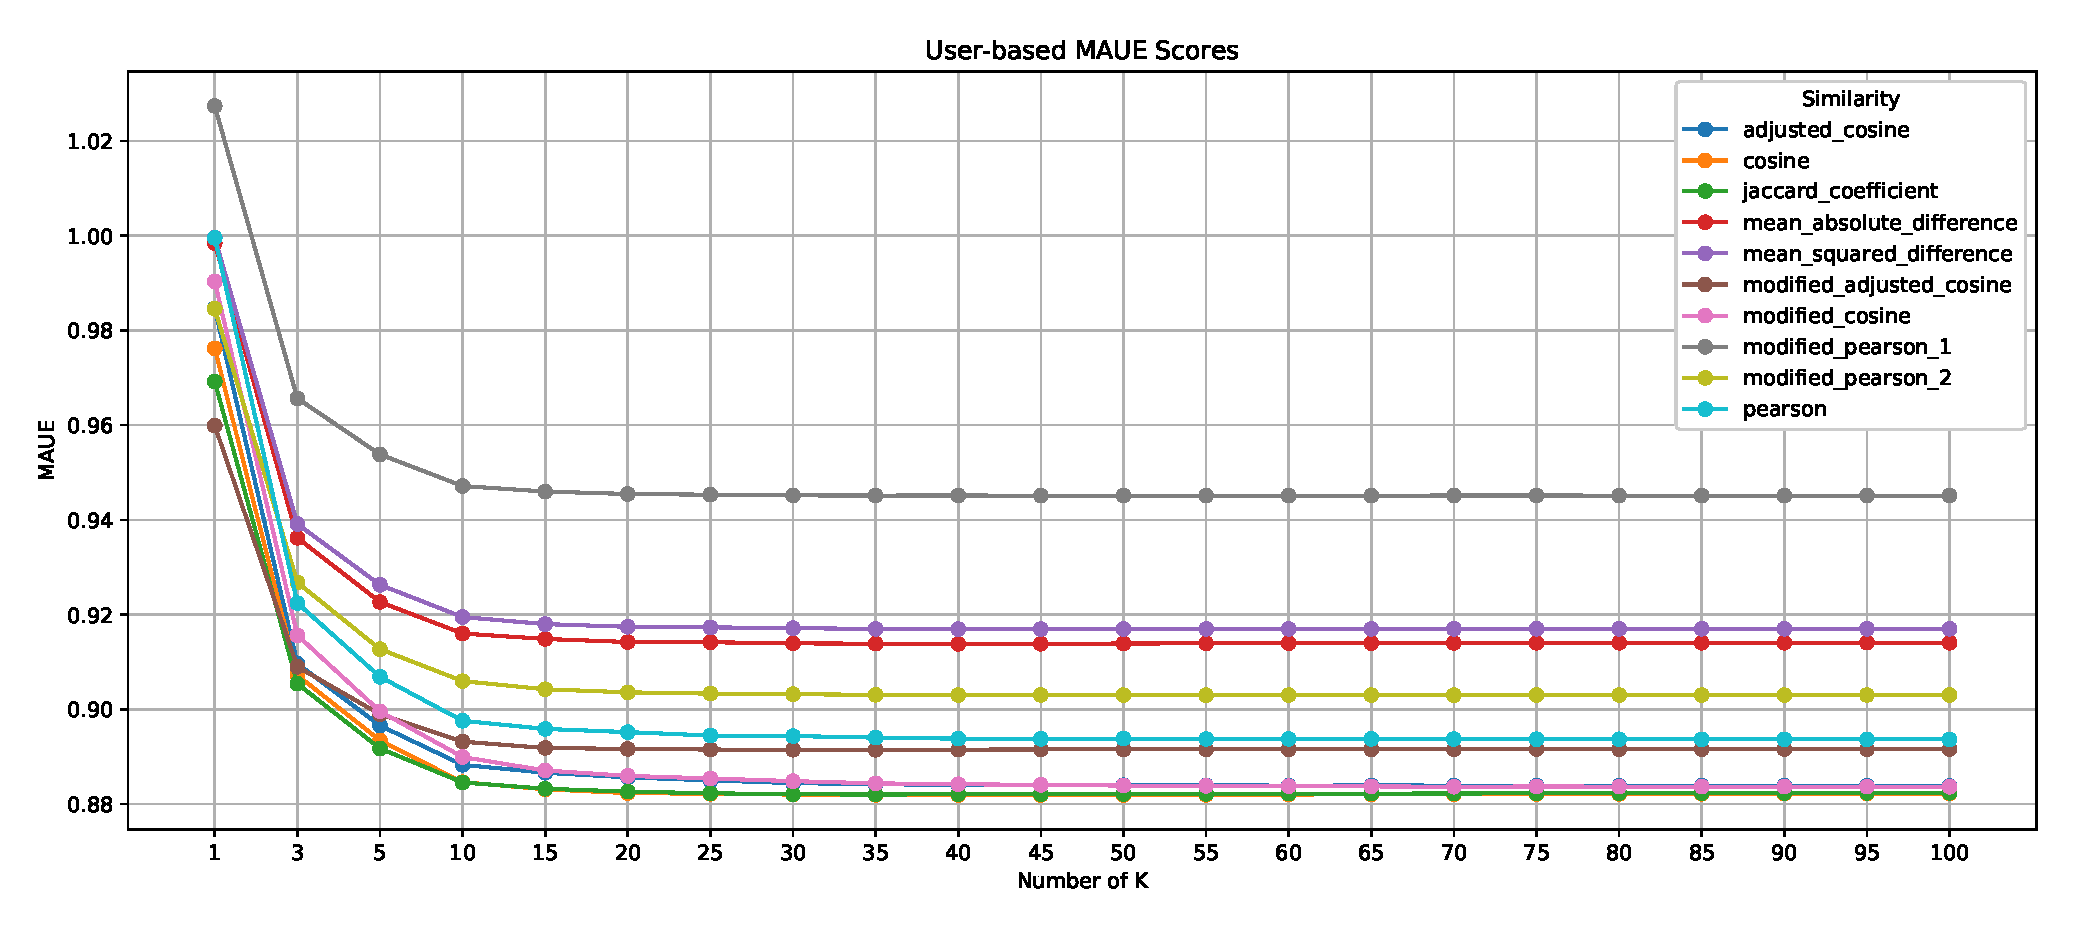
\includegraphics[width=1\textwidth]{chapter_4/knn/User_MAUE_KNN.eps}
\caption{User-based KNN MAUE Scores}
\label{figure:User_knn_maue}
\end{figure}

The best KNN MAUE score for user-based CF was produced using $\mathcal{K}=50$.
The exact KNN MAUE score is 0.8819077974 and it was calculated based on 100311 rating predictions(\autoref{table:prediction_counters_by_sim})
using the cosine similarity(\autoref{eq:cosine})
for the 144621 ratings in the test set(\autoref{table:epinions_descriptive}).

\begin{figure}[H]
\centering
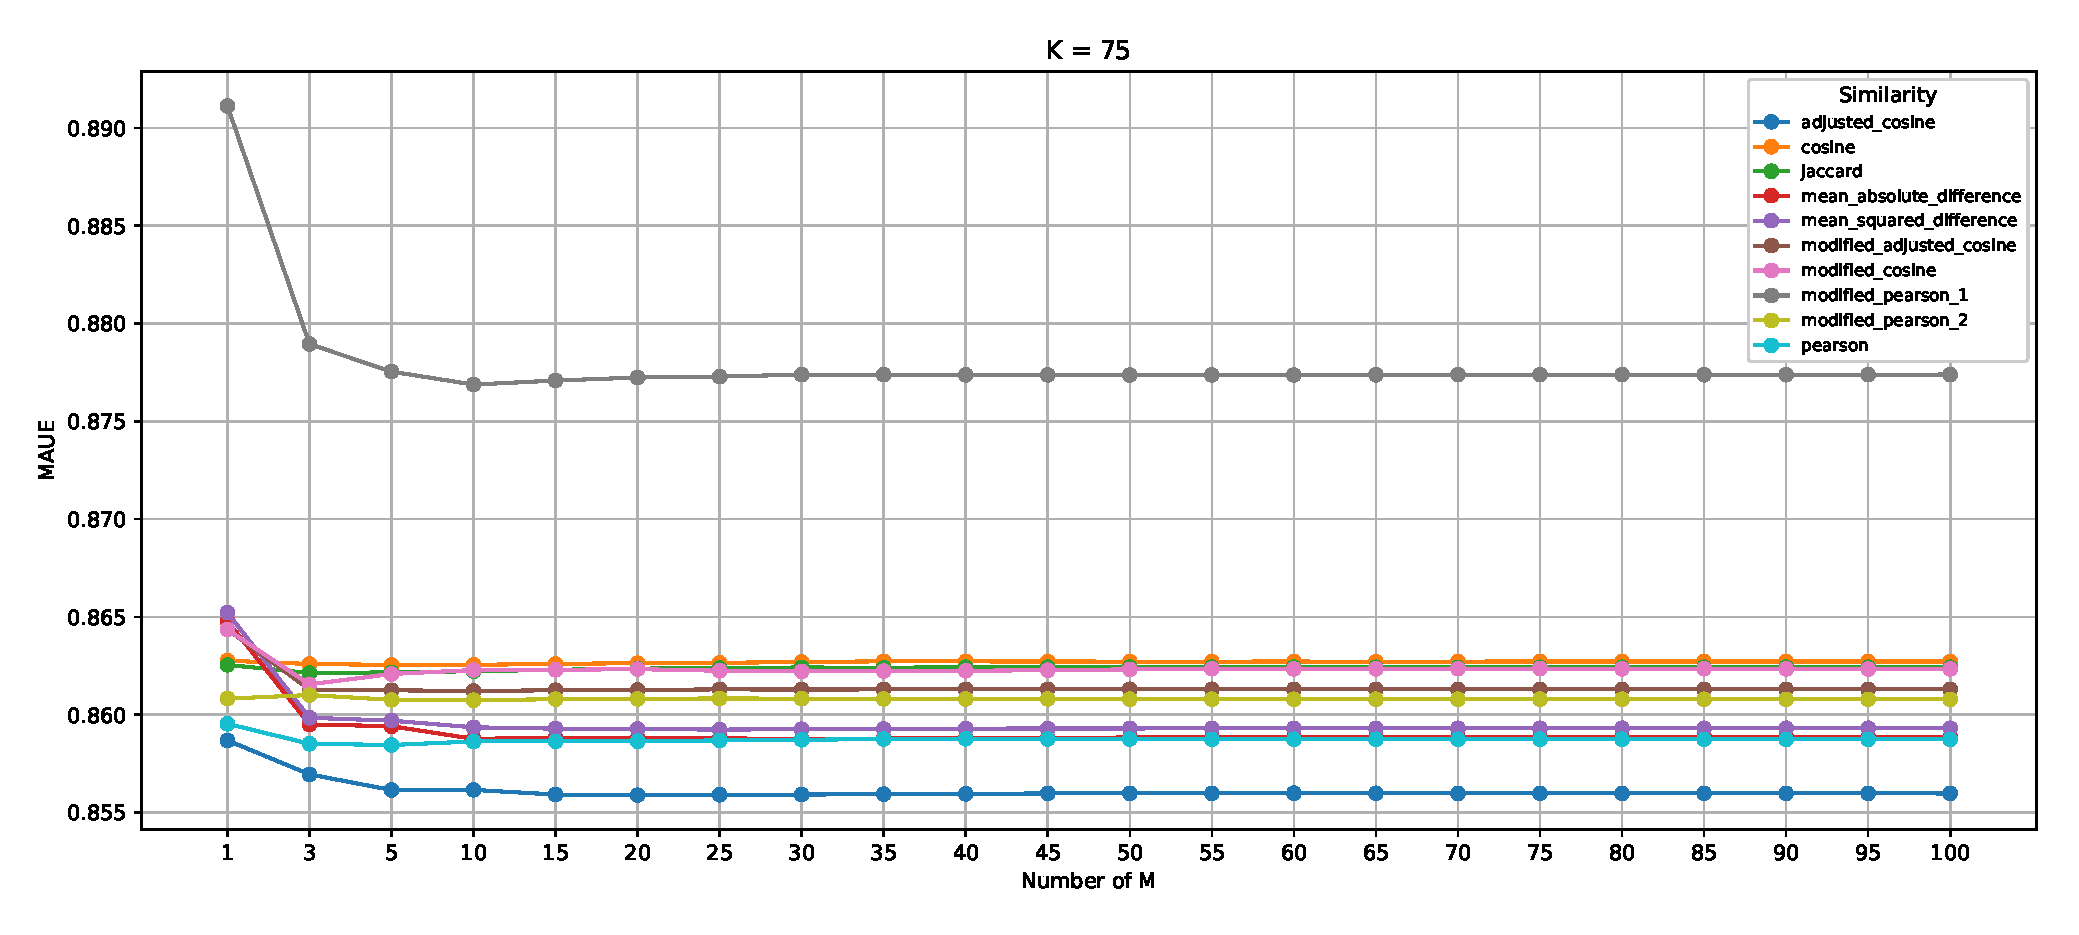
\includegraphics[width=1\textwidth]{chapter_4/evaluation/evaluation_user_maue.eps}
\caption{User-based Recursive-KNN MAUE Best Score}
\label{figure:User_rknn_maue}
\end{figure}

The best Recursive-KNN MAUE score for user-based CF was produced using $\mathcal{K}=75$ and \\$\mathcal{M}=20$.
The exact Recursive-KNN MAUE score is 0.8558869566 and it was calculated based on 34392 rating predictions(\autoref{table:prediction_counters_by_sim})
using the adjusted cosine similarity(\autoref{eq:adjusted_cosine})
out of the 36278 pairs for which KNN was unable to find neighbors(\autoref{table:users_log}).

\subsection{Item-based}
\begin{figure}[H]
\centering
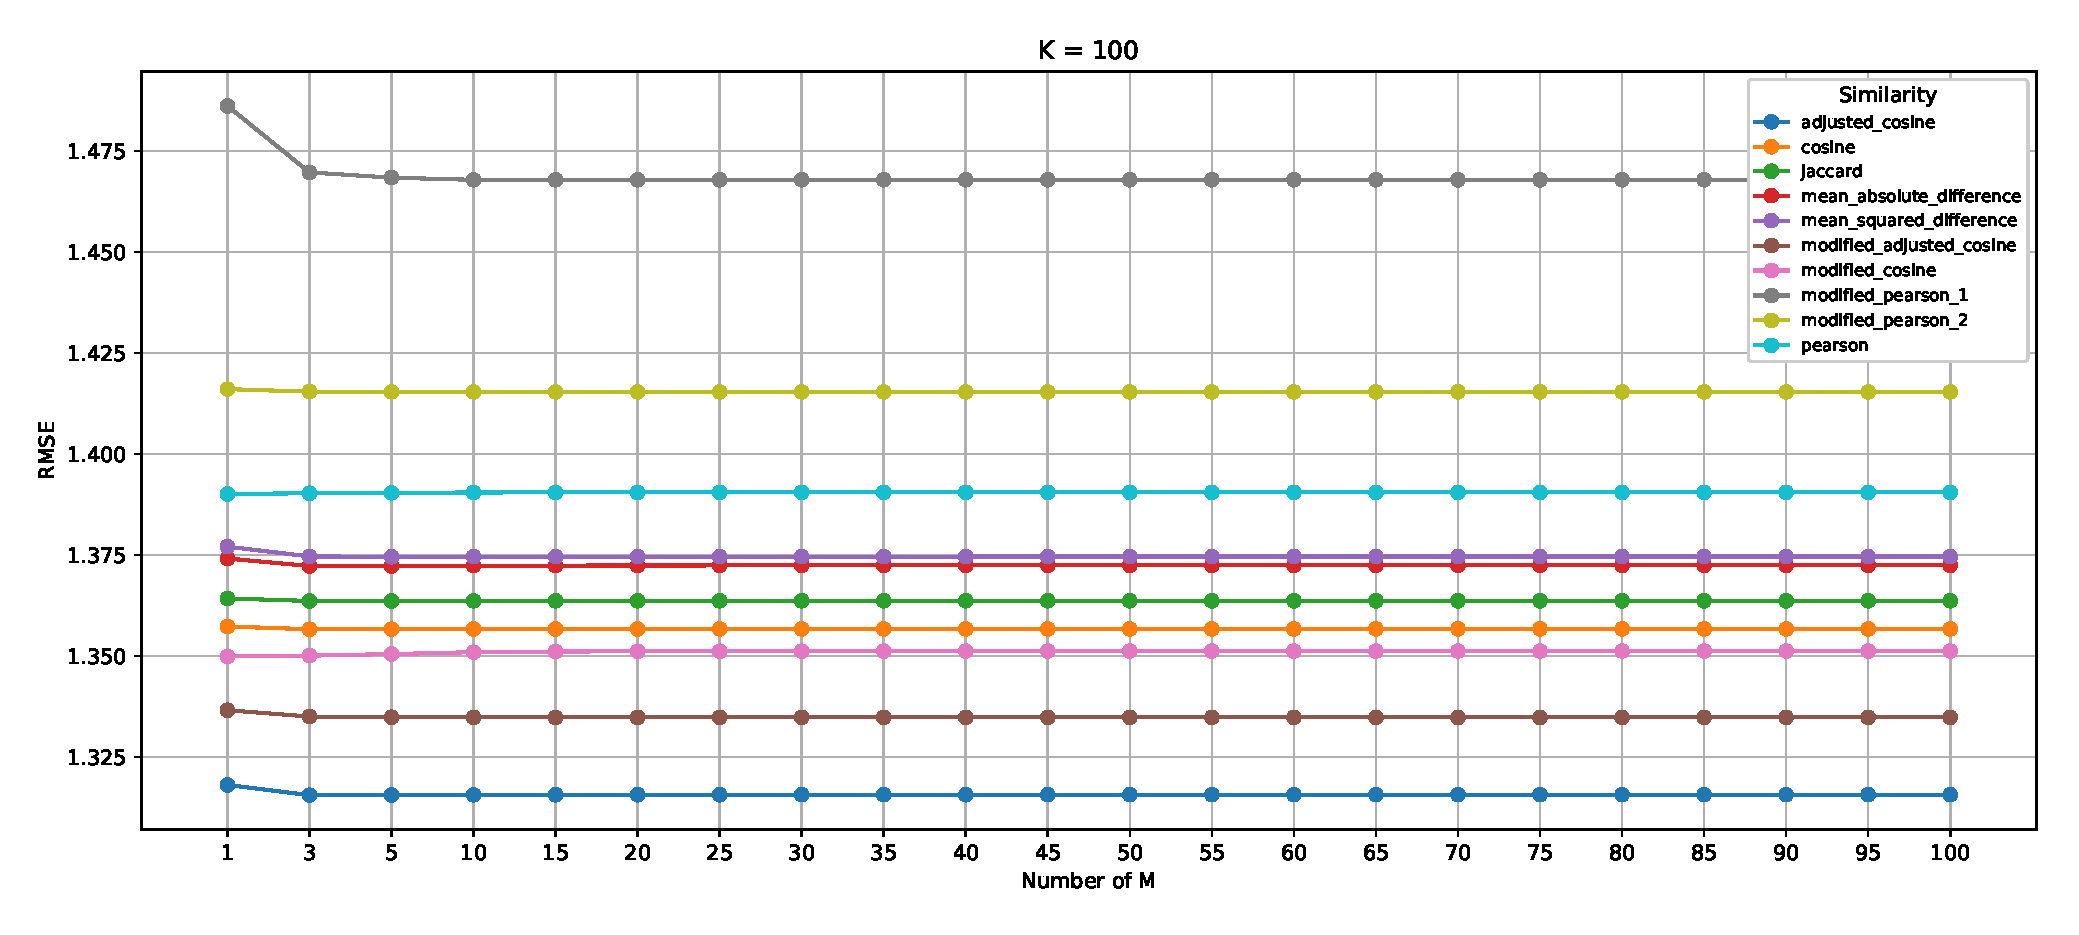
\includegraphics[width=1\textwidth]{chapter_4/evaluation/evaluation_item_rmse.eps}
\caption{Item-based Total RMSE Best Score}
\label{figure:Item_knn_rmse}
\end{figure}

The best RMSE score for item-based CF was produced using $\mathcal{K}=100$ and $\mathcal{M}=3$.
The exact RMSE score is 1.3155259043 and it was calculated based on 123115 rating predictions(\autoref{table:prediction_counters_by_sim})
using the adjusted cosine similarity(\autoref{eq:adjusted_cosine})
for the 144621 ratings in the test set(\autoref{table:epinions_descriptive}).

\begin{figure}[H]
\centering
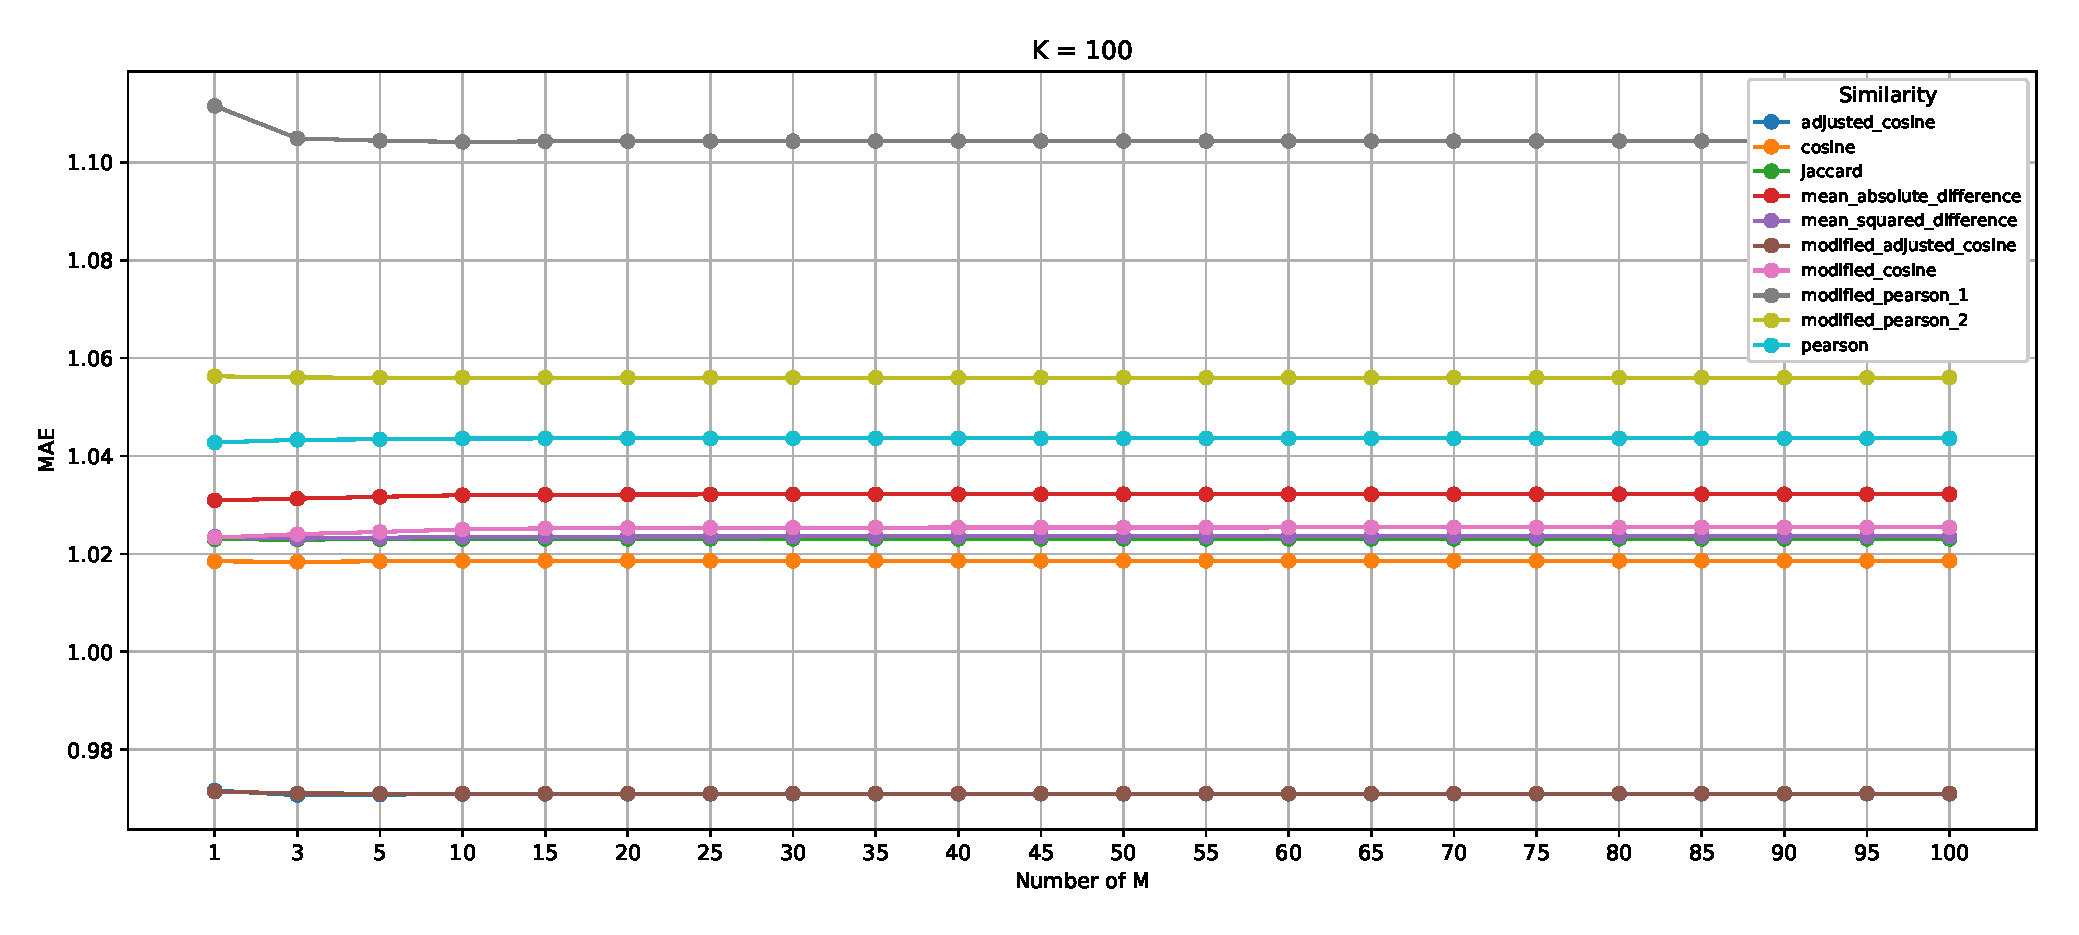
\includegraphics[width=1\textwidth]{chapter_4/evaluation/evaluation_item_mae.eps}
\caption{Item-based Total MAE Best Score}
\label{figure:Item_knn_mae}
\end{figure}

The best MAE score for item-based CF was produced using $\mathcal{K}=100$ and $\mathcal{M}=3$.
The exact MAE score is 0.9707211649 and it was calculated based on 123115 rating predictions(\autoref{table:prediction_counters_by_sim})
using the adjusted cosine similarity(\autoref{eq:adjusted_cosine})
for the 144621 ratings in the test set(\autoref{table:epinions_descriptive}).

\begin{figure}[H]
\centering
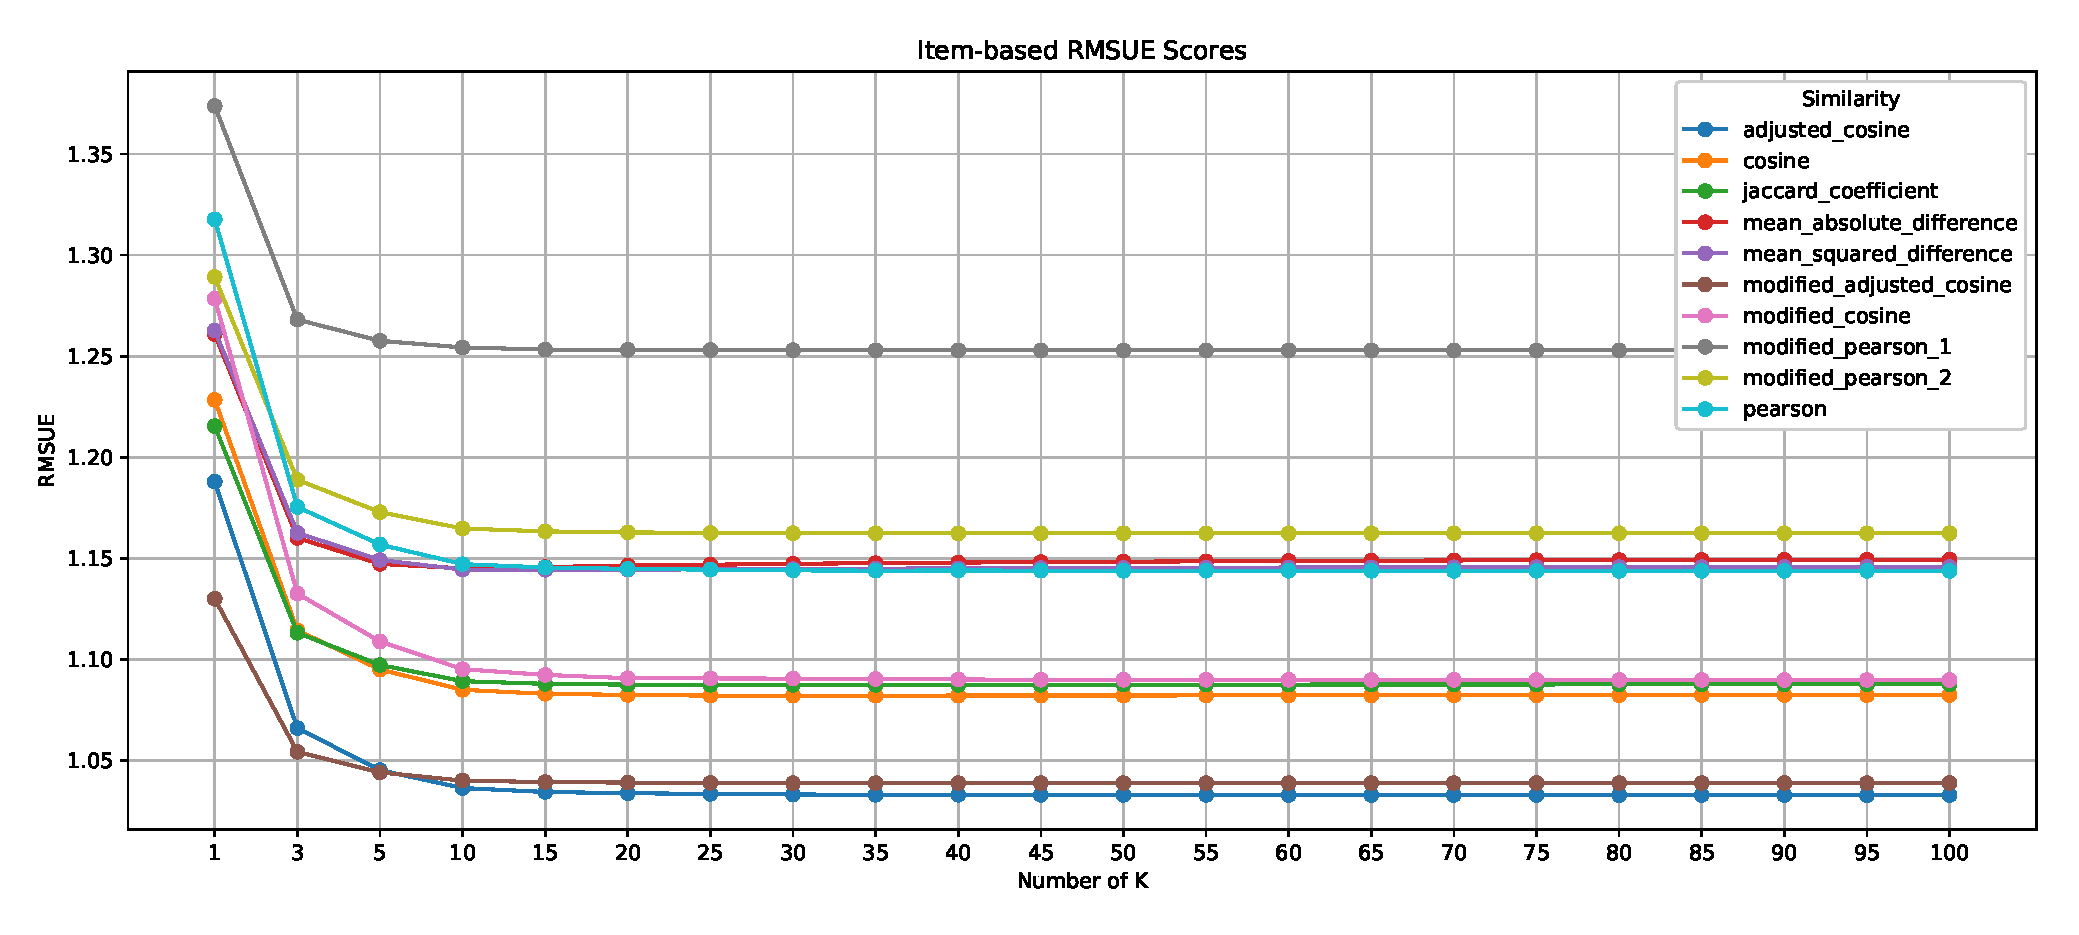
\includegraphics[width=1\textwidth]{chapter_4/knn/Item_RMSUE_KNN.eps}
\caption{Item-based KNN RMSUE Scores}
\label{figure:Item_knn_rmsue}
\end{figure}

The best KNN RMSUE score for item-based CF was produced using $\mathcal{K}=100$.
The exact KNN RMSUE score is 1.0328968801 and it was calculated based on 89800 rating predictions(\autoref{table:prediction_counters_by_sim})
using the adjusted cosine similarity(\autoref{eq:adjusted_cosine})
for the 144621 ratings in the test set(\autoref{table:epinions_descriptive}).

\begin{figure}[H]
\centering
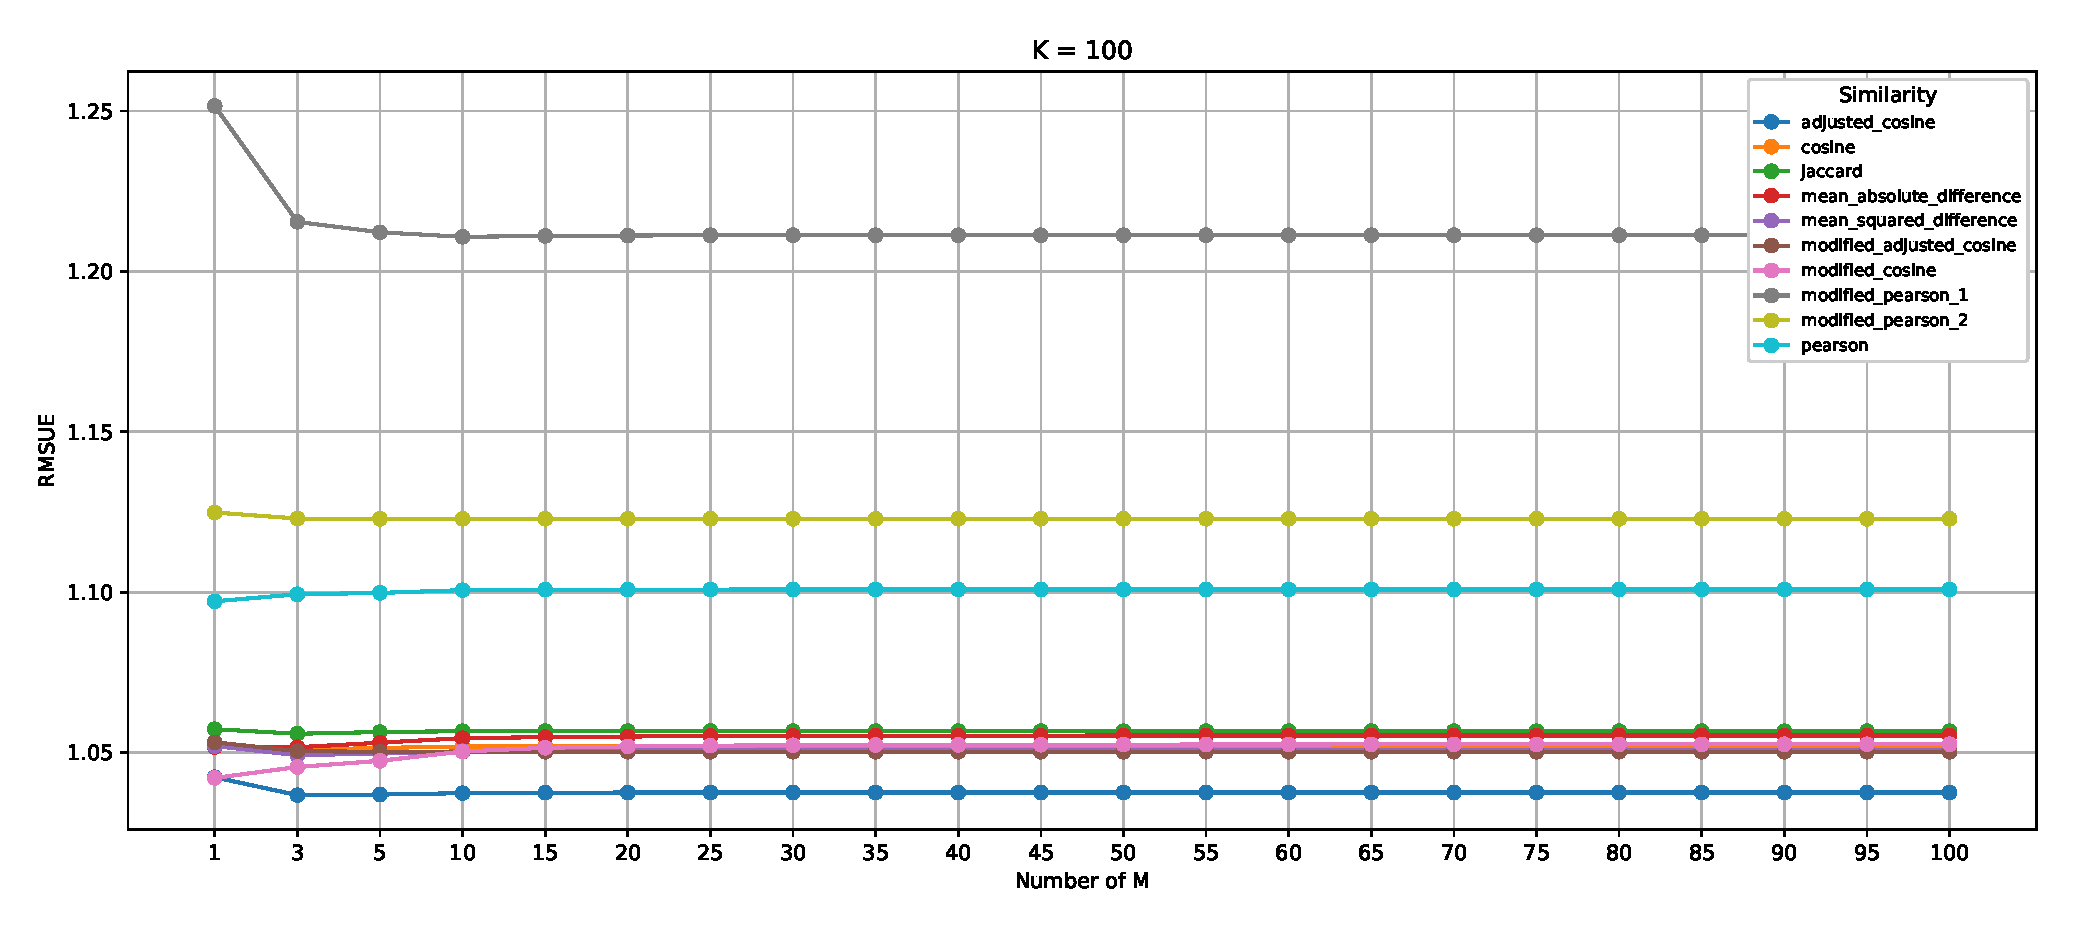
\includegraphics[width=1\textwidth]{chapter_4/evaluation/evaluation_item_rmsue.eps}
\caption{Item-based Recursive-KNN RMSUE Best Score}
\label{figure:Item_rknn_rmsue}
\end{figure}

The best Recursive-KNN RMSUE score for item-based CF was produced using $\mathcal{K}=100$ and $\mathcal{M}=3$.
The exact Recursive-KNN RMSUE score is 1.0367245756 and it was calculated based on 33315 rating predictions(\autoref{table:prediction_counters_by_sim})
using the adjusted cosine similarity(\autoref{eq:adjusted_cosine})
out of the 35280 pairs for which KNN was unable to find neighbors(\autoref{table:items_log}).

\begin{figure}[H]
\centering
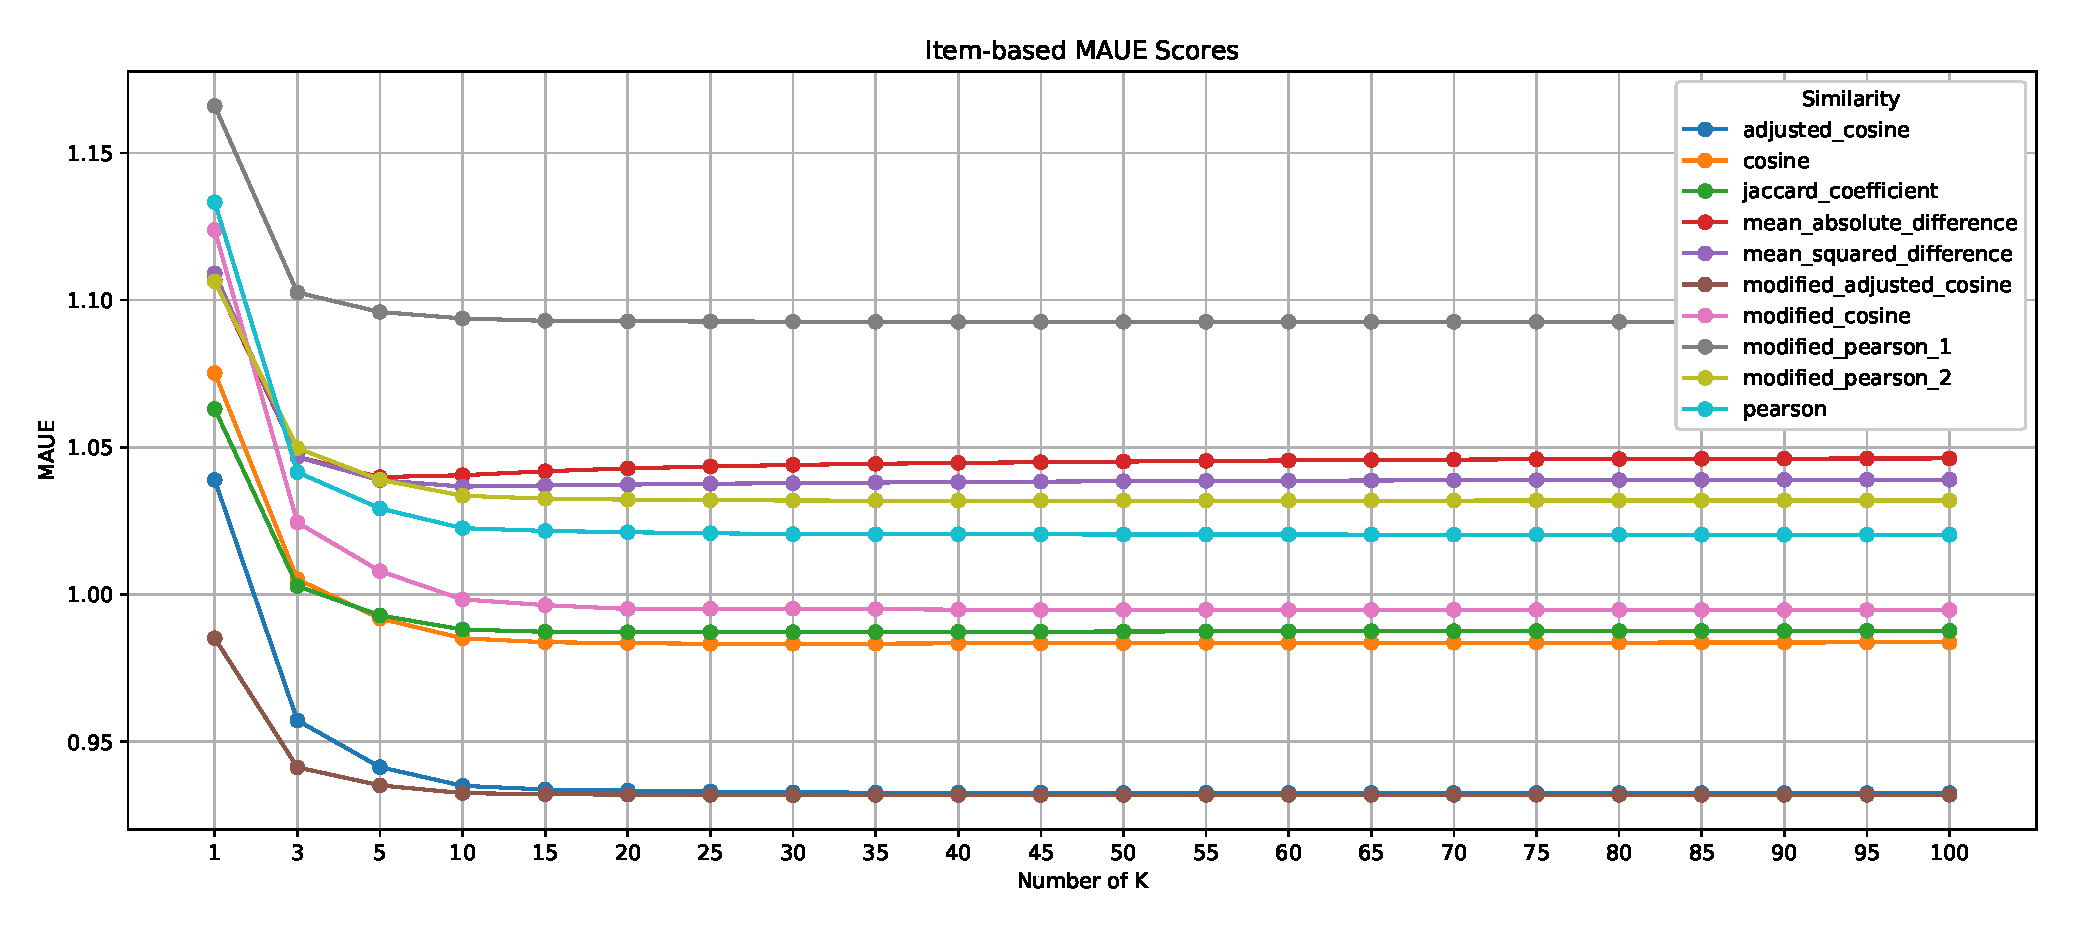
\includegraphics[width=1\textwidth]{chapter_4/knn/Item_MAUE_KNN.eps}
\caption{Item-based KNN MAUE Scores}
\label{figure:Item_knn_maue}
\end{figure}

The best KNN MAUE score for item-based CF was produced using $\mathcal{K}=30$.
The exact KNN MAUE score is 0.9318609947 and it was calculated based on 89800 rating predictions(\autoref{table:prediction_counters_by_sim})
using the modified adjusted cosine similarity(\autoref{eq:modified_adjusted_cosine})
for the 144621 ratings in the test set(\autoref{table:epinions_descriptive}).

\begin{figure}[H]
\centering
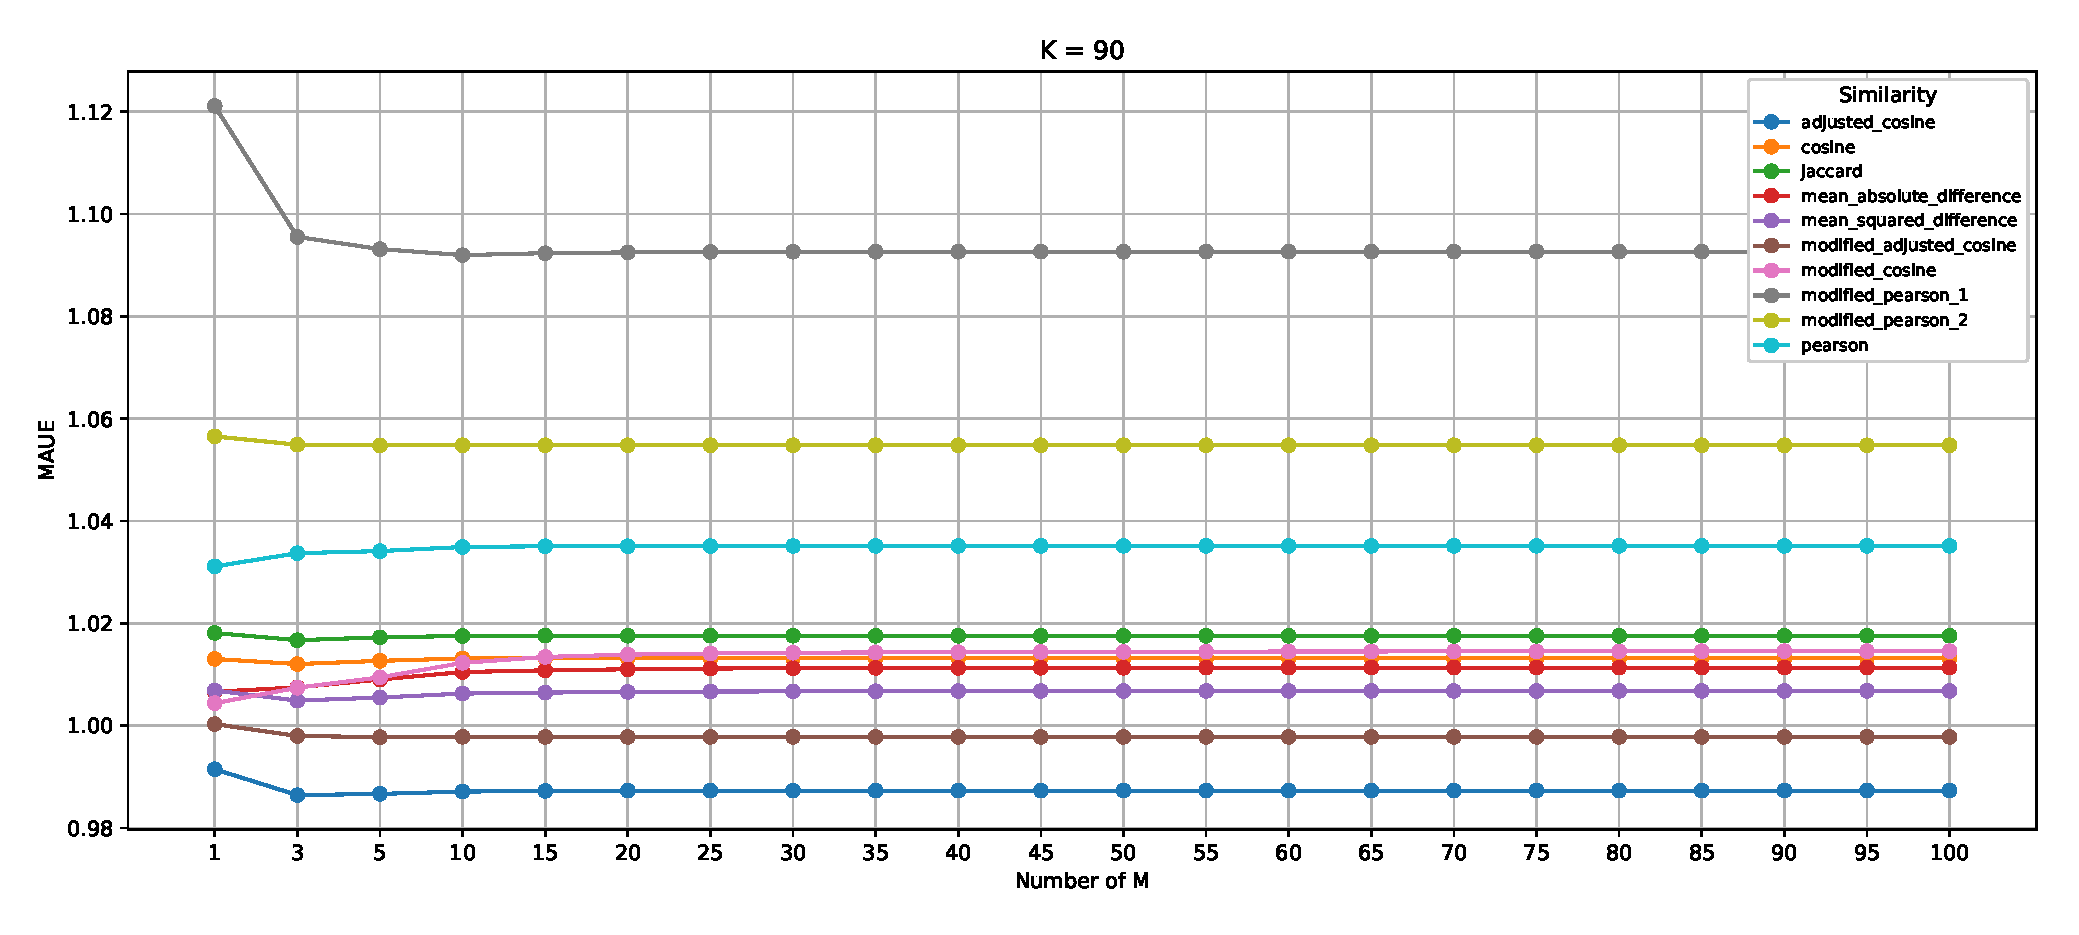
\includegraphics[width=1\textwidth]{chapter_4/evaluation/evaluation_item_maue.eps}
\caption{Item-based KNN MAUE Best Score}
\label{figure:Item_rknn_maue}
\end{figure}

The best Recursive-KNN MAUE score for item-based CF was produced using $\mathcal{K}=90$ and $\mathcal{M}=3$.
The exact Recursive-KNN MAUE score is 0.9864005988 and it was calculated based on 33315 rating predictions(\autoref{table:prediction_counters_by_sim})
using the adjusted cosine similarity(\autoref{eq:adjusted_cosine})
out of the 35280 pairs for which KNN was unable to find neighbors(\autoref{table:items_log}).

\subsection{Benchmarks}
\begin{table}[H]
\centering
\caption{Rating Predicted with KNN and Recursive-KNN}
\label{table:prediction_counters_by_sim}
\begin{tabular}{ccc|ccc|c}
\multicolumn{3}{c|}{\textbf{USERS}}            & \multicolumn{3}{c|}{\textbf{ITEMS}}            &                          \\ \cline{1-6}
\textbf{KNN} & \textbf{R-KNN} & \textbf{TOTAL} & \textbf{KNN} & \textbf{R-KNN} & \textbf{TOTAL} & \textbf{SIMILARITY}      \\ \hline
88379        & 34392          & 122771         & 89800        & 33315          & 123115         & Adjusted Cosine          \\
\textbf{100311}       & 24122          & \textbf{124433}         & \textbf{100311}       & 24122          & \textbf{124433}         & Cosine                   \\
\textbf{100311}       & 24122          & \textbf{124433}         & \textbf{100311}       & 24122          & \textbf{124433}         & Jaccard                  \\
93924        & 29747          & 123671         & 94528        & 29203          & 123731         & MAD                      \\
93924        & 29747          & 123671         & 94528        & 29203          & 123731         & MSD                      \\
88379        & 34392          & 122771         & 89800        & 33315          & 123115         & Modified Adjusted Cosine \\
\textbf{100311}       & 24122          & \textbf{124433}         & \textbf{100311}       & 24122          & \textbf{124433}         & Modified Cosine          \\
59017        & \textbf{40470}          & 99487          & 54644        & \textbf{34096}          & 88740          & Modified Pearson 1       \\
89936        & 28183          & 118119         & 84511        & 24357          & 108868         & Modified Pearson 2       \\
89936        & 28183          & 118119         & 84511        & 24357          & 108868         & Pearson
\end{tabular}
\end{table}

Cosine, Jaccard and Modified Cosine were able to produce the most rating predictions, 124433 in total,
both for user-based and item-based. Modified Pearson 1 was the one with the least similarities
(\autoref{table:modified_pearson_1_descriptive}) and therefore the one with the least rating
predictions, even though, it managed to predict a total of 99487 ratings user-based
and 88740 item-based. The outcome however was very poor for this similarity formula for any
evaluation metric. The average boost in rating predictions using the Recursive-KNN method was
about 25\% for user-based CF and 24\% for item-based CF.
\newpage
The two tables below are the logs produced for user-based(\autoref{table:users_log})
and item-based(\autoref{table:items_log}) KNN and Recursive-KNN algorithms.
The first three columns refer to the KNN algorithm and present the number of pairs that KNN
algorithm was unable to predict. The first column indicates the number of pairs
(user, item) for which relevant nearest neighbors did not exist. The second column
indicates the number of pairs that either the item in user-based or user in
item-based did not exist in the train set. The third column indicates the number
of pairs that either the user in user-based or item in
item-based did not exist in the train set and therefore KNN could not find similarities.
The test was for 22 different values of $\mathcal{K}$. The total compute time for each similarity
metric for all $\mathcal{K}$'s is indicated in the fourth column.
The next two columns refer to Recursive-KNN algorithm. The fifth column indicates
the number of pairs that could not be predicted due to no further neighbors
after the completion of the Recursive-KNN algorithm.
The sixth column is the time the Recursive-KNN took for completing all the available combinations
484 in count between $\mathcal{K}$'s and $\mathcal{M}$'s (i.e. ($\mathcal{M}$=1, $\mathcal{K}$=1),
($\mathcal{M}$=1, $\mathcal{K}$=3), ($\mathcal{M}$=3, $\mathcal{K}$=1) e.t.c.).

The computations were run on a cloud computing platform.
The specifications of the machine were the following:
\begin{itemize}
	\item[] \textbf{OS:} Ubuntu Server 16.04.3
	\item[] \textbf{CPU:} Intel Xeon E5-2697A v4 @ 2.60GHz
	\item[] \textbf{RAM:} 3GB DDR4 + 1GB SWAP
\end{itemize}

\begin{table}[H]
\centering
\caption{User-based KNN and Recursive-KNN Log}
\label{table:users_log}
\begin{tabular}{|c|c|c|c|c|c|c|}
\cline{1-6}
\multicolumn{4}{|c|}{\textbf{KNN}}                                               & \multicolumn{2}{c|}{\textbf{Recursive-KNN}} & \multicolumn{1}{l}{}                          \\ \hline
\textbf{No NN} & \textbf{Not in Train} & \textbf{No Similarity} & \textbf{Time} & \textbf{R-No NN} & \textbf{R-Time}		& \multicolumn{1}{c|}{\textbf{Similarity}}      \\ \hline
36278          & 18939                 & 1025                  & 0:3:58        & 1886             & 4:3:9           		& \multicolumn{1}{c|}{adjusted cosine}          \\ \hline
25061          & 18939                 & 310                   & 0:5:17        & 939              & 4:1:57          		& \multicolumn{1}{c|}{cosine}                   \\ \hline
25061          & 18939                 & 310                   & 0:3:41        & 939              & 2:57:58         		& \multicolumn{1}{c|}{jaccard}                  \\ \hline
31200          & 18939                 & 558                   & 0:4:16        & 1453             & 3:2:29          		& \multicolumn{1}{c|}{mad}                      \\ \hline
31200          & 18939                 & 558                   & 0:4:9         & 1453             & 3:9:12          		& \multicolumn{1}{c|}{msd}                      \\ \hline
36278          & 18939                 & 1025                  & 0:4:13        & 1886             & 4:3:56          		& \multicolumn{1}{c|}{modified adjusted cosine} \\ \hline
25061          & 18939                 & 310                   & 0:4:31        & 939              & 2:42:42         		& \multicolumn{1}{c|}{modified cosine}          \\ \hline
48886          & 18939                 & 17779                 & 0:3:8         & 8416             & 1:33:26         		& \multicolumn{1}{c|}{modified pearson 1}       \\ \hline
29450          & 18939                 & 6296                  & 0:3:18        & 1267             & 3:4:17          		& \multicolumn{1}{c|}{modified pearson 2}       \\ \hline
29450          & 18939                 & 6296                  & 0:3:8         & 1267             & 2:48:48         		& \multicolumn{1}{c|}{pearson}                  \\ \hline
\end{tabular}
\end{table}

\begin{table}[H]
\centering
\caption{Item-based KNN and Recursive-KNN Log}
\label{table:items_log}
\begin{tabular}{|c|c|c|c|c|c|c}
\cline{1-6}
\multicolumn{4}{|c|}{\textbf{KNN}}                                               & \multicolumn{2}{c|}{\textbf{Recursive-KNN}} & \multicolumn{1}{l}{}                          \\ \hline
\textbf{No NN} & \textbf{Not in  Train} & \textbf{No Similarity} & \textbf{Time} & \textbf{R-No NN}      & \textbf{R-Time}     & \multicolumn{1}{c|}{\textbf{Similarity}}      \\ \hline
35280          & 0                      & 19541                  & 0:3:2         & 1965                  & 2:18:35             & \multicolumn{1}{c|}{adjusted cosine}          \\ \hline
25188          & 0                      & 19122                  & 0:3:43        & 1066                  & 2:26:56             & \multicolumn{1}{c|}{cosine}                   \\ \hline
25188          & 0                      & 19122                  & 0:3:37        & 1066                  & 2:12:56             & \multicolumn{1}{c|}{jaccard}                  \\ \hline
30827          & 0                      & 19266                  & 0:3:22        & 1624                  & 1:54:18             & \multicolumn{1}{c|}{mad}                      \\ \hline
30827          & 0                      & 19266                  & 0:3:28        & 1624                  & 1:58:50             & \multicolumn{1}{c|}{msd}                      \\ \hline
35280          & 0                      & 19541                  & 0:3:10        & 1965                  & 2:32:4              & \multicolumn{1}{c|}{modified adjusted cosine} \\ \hline
25188          & 0                      & 19122                  & 0:3:37        & 1066                  & 2:11:18             & \multicolumn{1}{c|}{modified cosine}          \\ \hline
41037          & 0                      & 48940                  & 0:2:14        & 6941                  & 0:39:1              & \multicolumn{1}{c|}{modified pearson 1}       \\ \hline
25332          & 0                      & 34778                  & 0:2:58        & 975                   & 1:49:35             & \multicolumn{1}{c|}{modified pearson 2}       \\ \hline
25332          & 0                      & 34778                  & 0:2:52        & 975                   & 1:46:24             & \multicolumn{1}{c|}{pearson}                  \\ \hline
\end{tabular}
\end{table}
